\section{\Large PROBLEM SET 6}

\subsection{Problem 1 - Complete the modeling and verification of perturbation torques as described in the previous pset} \label{sec:pertTorques}

In the previous problem set, the magnetic torque was implemented successfully, but the aerodynamic and solar radiation torques still needed improvement. For the solar radiation torque, the unit vector pointing towards the sun needed to be implemented. To accomplish this, the orbit propagator used for the satellite was leveraged. The propagator was modified to take in the orbital elements of the desired orbit at the beginning of the simulation such that it could be called separately for the satellite and the sun. The new resultant layout of the simulink file is shown below in Figure \ref{fig:sun_orbit_sim}.

\begin{figure}[H]
    \centering
    \captionsetup{ justification = centering }
    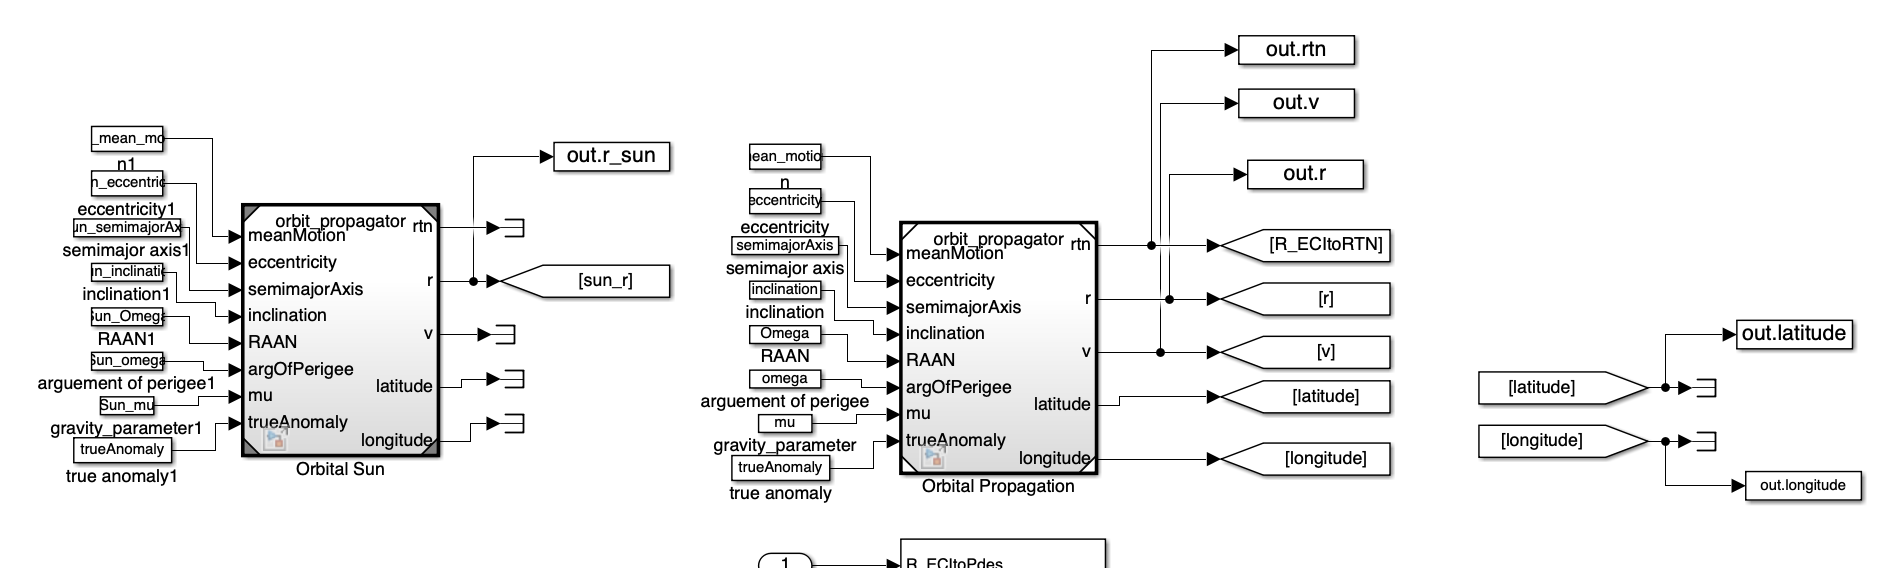
\includegraphics[width = 12cm]{Images/PS6/updatedOrbitPropagatorSim.png}
    \caption{Updated Orbit Propagator to include Sun Orbit Propagation}
    \label{fig:sun_orbit_sim}
\end{figure}

In the above simulink model, the orbital elements of Earth's orbit around the sun were used to simulate the 'orbit' of the sun around the Earth in the ECI frame. The semimajor axis and eccentricity were left untouched as they are independent of coordinate frames. It is important to note, however, that the angular values including the inclination were adjusted to be in Earth's equatorial plane that is offset by the ecliptic plane by 23.5$\degree$. The orbital parameters that were used are shown below.

\begin{center}
    a = 7080.6 km \\
    e = 0.0000979 \\
    i = 98.2$\degree$ \\
    $\Omega$ = 95.2063$\degree$ \\
    $\omega$ = 120.4799$\degree$ \\
\end{center}

A plot showing the resultant orbit of the sun 'around' the Earth is shown below in Figure \ref{fig:sun_orbit}.

\begin{figure}[H]
    \centering
    \captionsetup{ justification = centering }
    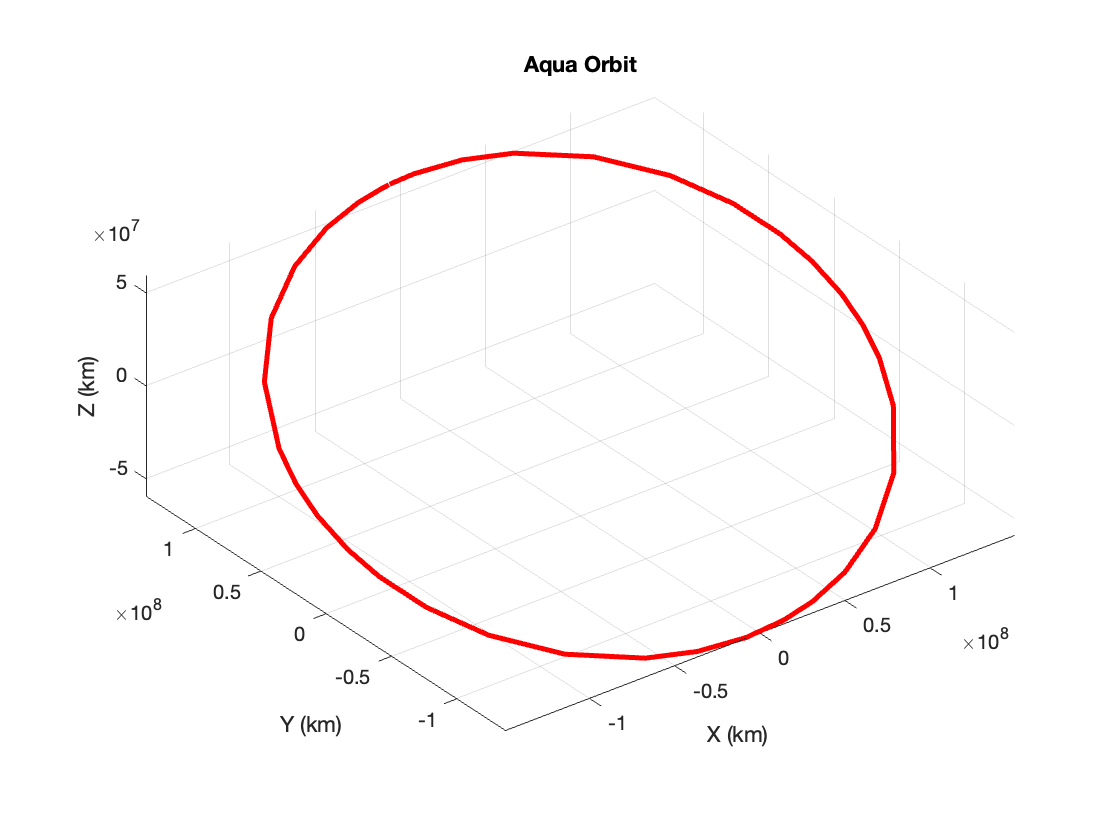
\includegraphics[width = 12cm]{Images/PS6/sunOrbit.png}
    \caption{Orbit of the Sun Around Earth in ECI Frame}
    \label{fig:sun_orbit}
\end{figure}

One it was verified that the unit vector pointing towards the sun was correct, the remaining tasks for the solar radiation torque were finding values for $c_d$ and $c_s$ that aligned with the theory and approximating the center of pressure of the satellite. While the exact materials used for the Aqua satellite are unknown, it is safe to assume that the solar array had a lower $c_d$ value than the encasing of the sensors and electronics in the satellite. This is because the encasing is typically covered in an opaque white paint to protect the electronics from environmental dangers. Therefore, $c_d$ was adjusted to be high for every surface except the two designated to the solar array and $c_1$ followed the opposite relationship to ensure that $c_d + c_s < 1$. Finally, the center of pressure was calculated through the following approximation.

\begin{equation}
    \frac{\sum^n_{i=1} A_i c_i}{\sum^n_{i=1} A_i}
\end{equation}

In this equation A represents the area of each surface and c represents the centroid location in the principle frames. Through making these corrections and debugging small issues in the simulink model shown in Figure \ref{fig:simulink_sol}. The resultant torques plotted versus time are shown in Figure \ref{fig:solar_torque}.

\begin{figure}[H]
    \centering
    \captionsetup{ justification = centering }
    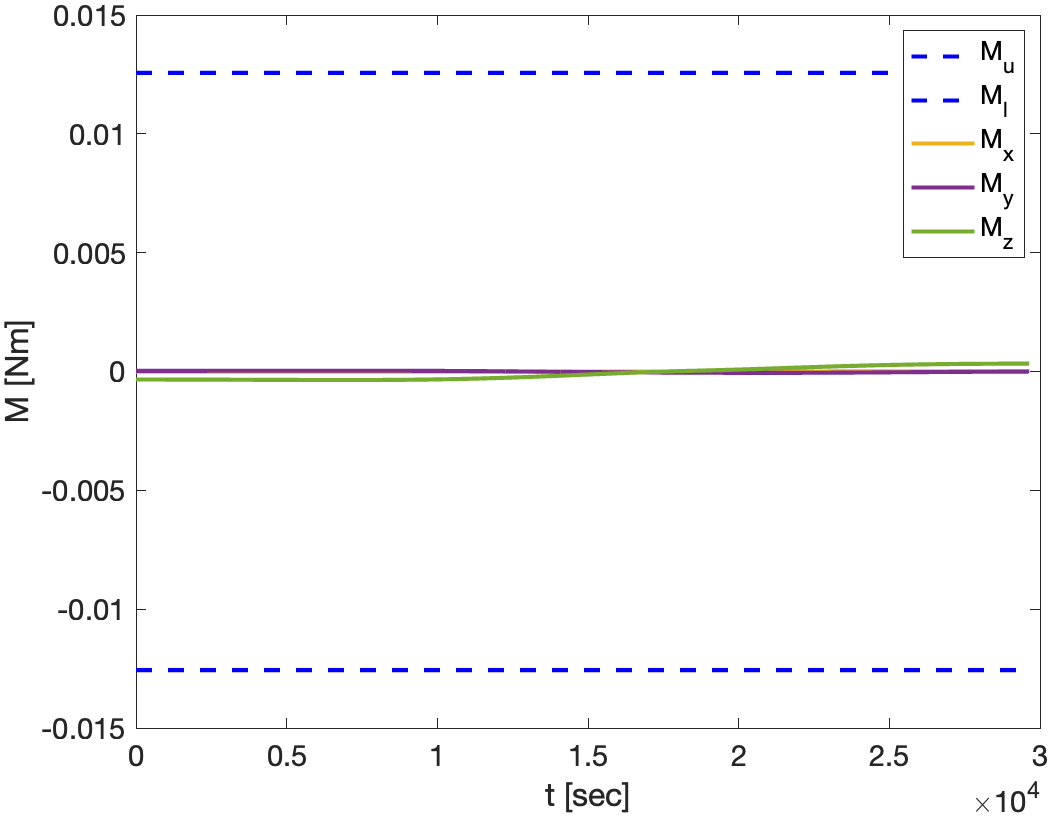
\includegraphics[width = 12cm]{Images/PS6/solar_torque.png}
    \caption{Solar Torque}
    \label{fig:solar_torque}
\end{figure}

The small oscillations shown in Figure \ref{fig:solar_torque} confirm that the torque is periodic for the Earth pointing satellite as predicted in theory. Furthermore, the torque is well within the bounds. 

For the aerodynamic drag, the theory shown in last weeks problem set was correct, but small issues needed to be debugged with the model. Once these bugs were resolved, the resultant torques were obtained and are shown below in Figure \ref{fig:aero_torque}.

\begin{figure}[H]
    \centering
    \captionsetup{ justification = centering }
    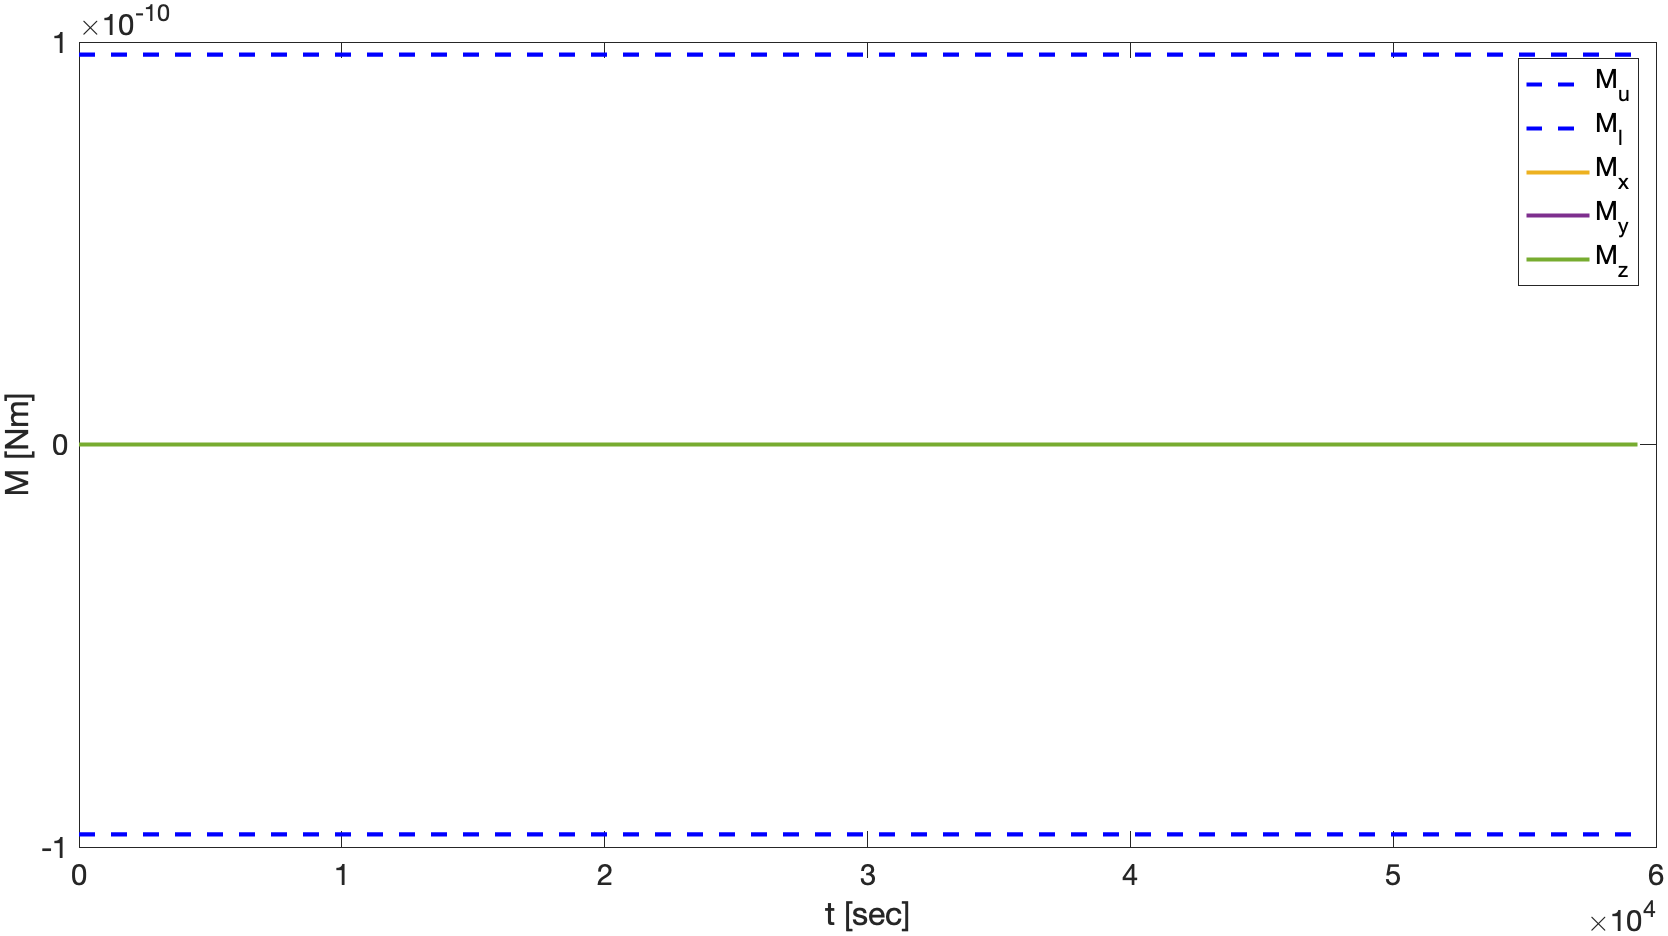
\includegraphics[width = 12cm]{Images/PS6/aero_torque.png}
    \caption{Aerodynamic Torque}
    \label{fig:aero_torque}
\end{figure}


As predicted in the theory, the drag is constant for the earth pointing satellite, and stays well within the bounds thus validating the simulation. Finally, once all of the disturbances were obtained, they were combined to obtain the total torque from aerodynamic drag, solar radiation, gravity, and magnetic disturbances. The total torque is shown below in Figure \ref{fig:all_torque}.

\begin{figure}[H]
    \centering
    \captionsetup{ justification = centering }
    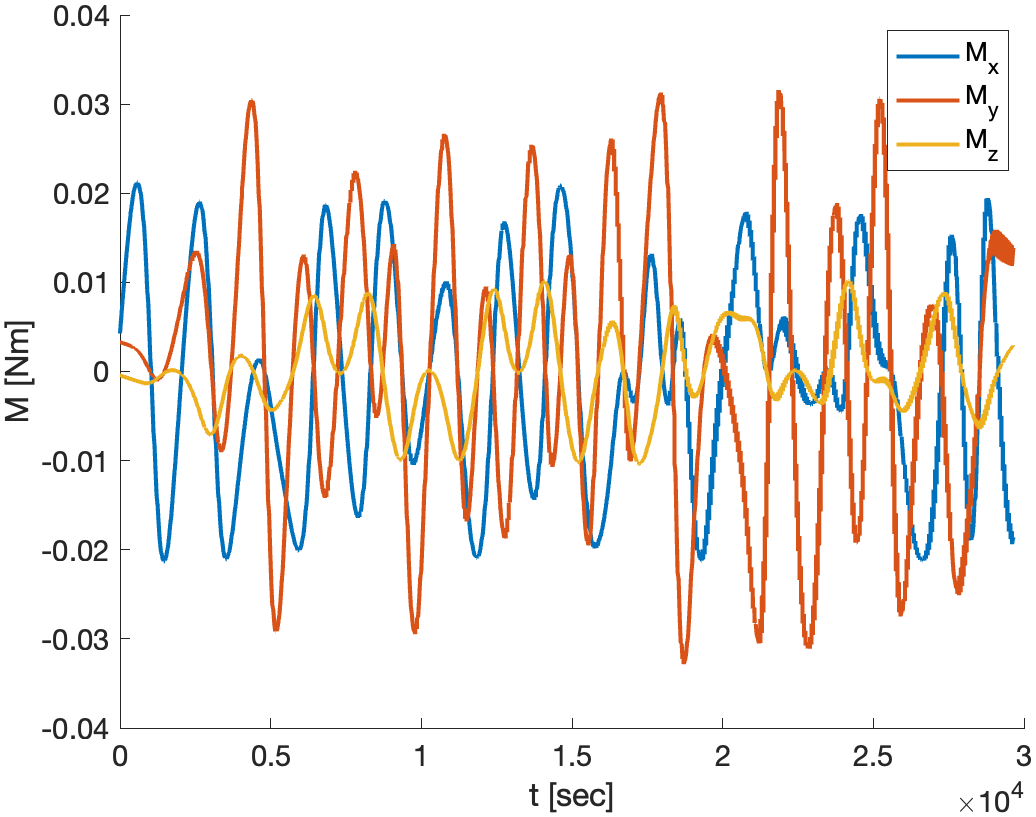
\includegraphics[width = 12cm]{Images/PS6/all_torque.png}
    \caption{Total Torque}
    \label{fig:all_torque}
\end{figure}

The total torque shows that the primary disturbance contributors are gravity and solar radiation for our satellite and its mission. 

\subsection{Problem 2 - Compute the attitude control error even if a controller is not implemented yet. The attitude control error represents the rotation between the desired and actual attitude. Plot the attitude control error and give its interpretation. Note that this step requires the definition and computation of the desired or nominal or target attitude of the spacecraft. In general, this can be expressed in body or principal axes.}

Recall that the mission for the Aqua satellite requires the instruments on the bottom of the spacecraft to be Earth-pointing. With the selected body axes, this means that the desired attitude expressed as a rotation matrix from the RTN frame to the body frame is described as follows.

\begin{equation*}
    \boldsymbol{\bar{R}}_{RTN \rightarrow x'y'z'} = \begin{bmatrix}
        0 & 1 & 0 \\ 0 & 0 & 1 \\ 1 & 0 & 0
    \end{bmatrix}
\end{equation*}

To get the desired orientation of the principal frame we use the rotation described in Section \ref{sec:principal_inertia_def_and_calc}. Using Equation \ref{eq:desired_principal_RTN}, the desired attitude of the principal frame with respect to the RTN frame can computed, where $\boldsymbol{A}$ is represented by $\boldsymbol{R}_{xyz \rightarrow x'y'z'}$.

\begin{equation} \label{eq:desired_principal_RTN}
    \boldsymbol{\bar{R}}_{RTN \rightarrow xyz} = \boldsymbol{R}_{xyz \rightarrow x'y'z'}^T \boldsymbol{\bar{R}}_{RTN \rightarrow x'y'z'}
\end{equation}

Therefore, at each step in the simulation, the desired attitude with respect to the ECI frame is computed using Equation \ref{eq:desired_principal_ECI}.

\begin{equation} \label{eq:desired_principal_ECI}
    \boldsymbol{\bar{R}}_{ECI \rightarrow xyz} = \boldsymbol{\bar{R}}_{RTN \rightarrow xyz} \boldsymbol{R}_{ECI \rightarrow RTN}
\end{equation}

The error between the current and desired attitude can be represented by a rotation from the current attitude to the desired attitude. This rotation can be computed using Equation \ref{eq:error_rotation}

\begin{equation} \label{eq:error_rotation}
    \boldsymbol{R}_{\text{error}} = \boldsymbol{R}_{xyz \rightarrow \overline{xyz}} = \boldsymbol{\bar{R}}_{ECI \rightarrow xyz} \boldsymbol{R}_{ECI \rightarrow xyz}^T
\end{equation}

Aligning the satellite initially with this initial condition but giving it no initial angular velocity should yield an evolution of the error that mostly resembles a linear increase in the angle $\theta$. This is because this angle represents the error about the desired 2-axis, which in our desired alignment corresponds to the N-axis in the RTN frame. In the absence of disturbances the only apparent rotation should be that of the RTN frame as the satellite moves in its orbit. Figure \ref{fig:attitude_error_no_dist} corroborates this interpretation. An issue occurs with a singularity at $\theta = 90^\circ$, causing the signs of the other two angles to flip. The general behavior, however, remains the same under this consideration.

\begin{figure}[H]
    \centering
    \captionsetup{ justification = centering }
    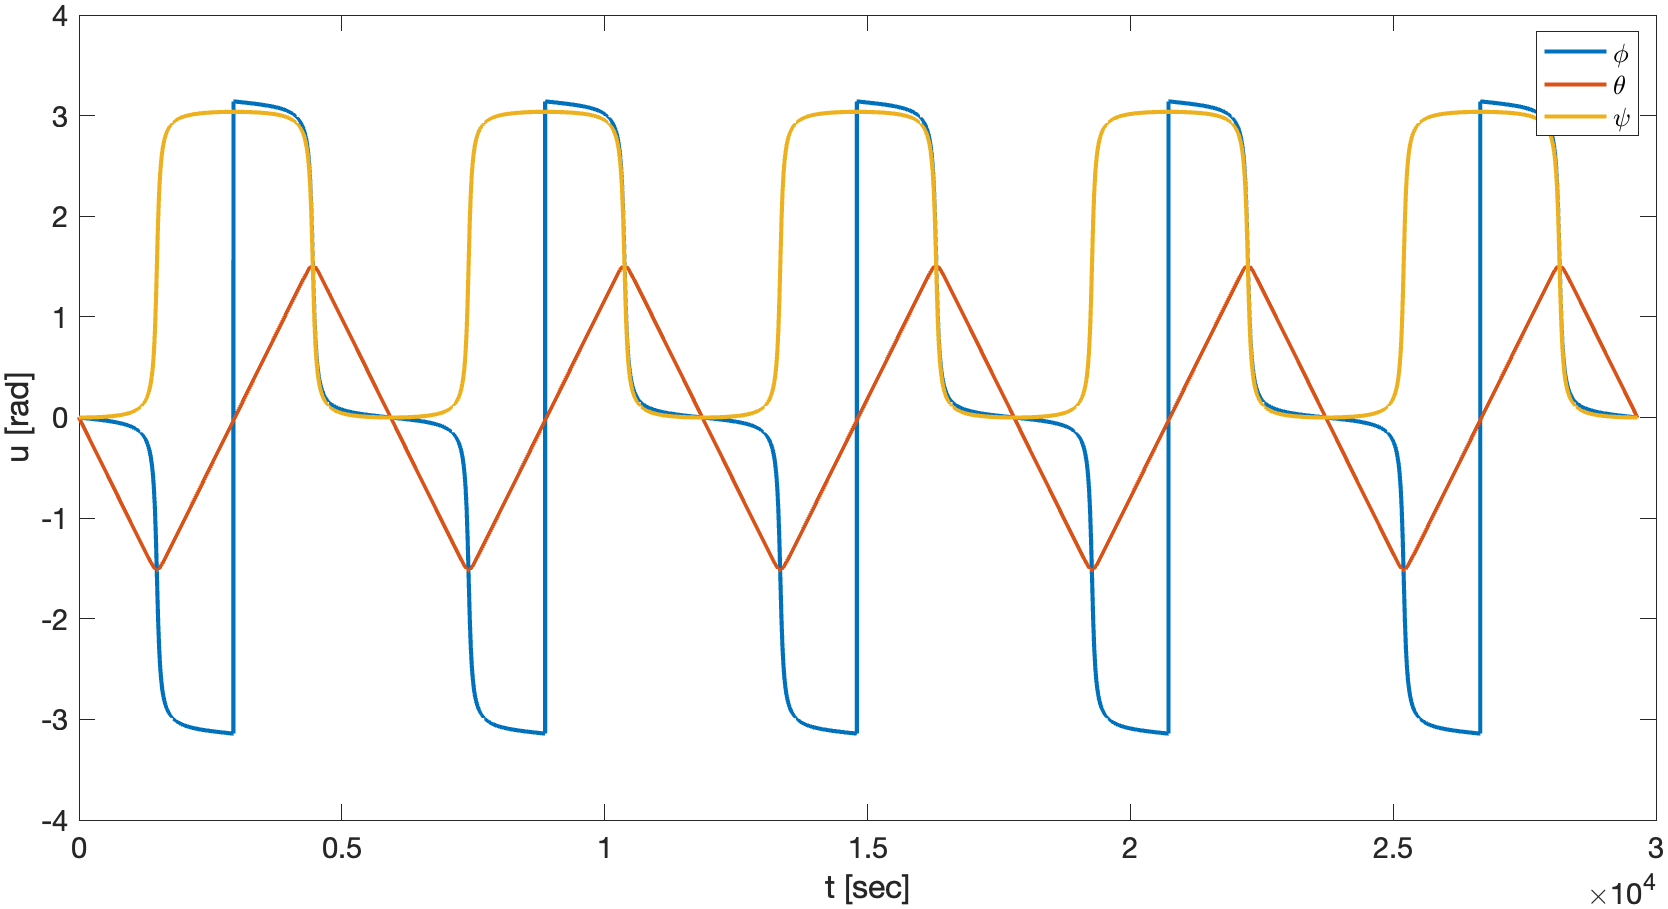
\includegraphics[width = 12cm]{Images/PS6/attitude_error_no_dist.png}
    \caption{312 Euler Angle Parameterization of the Rotation Error in the Absence of Disturbance Torques}
    \label{fig:attitude_error_no_dist}
\end{figure}

\subsection{Problem 3 - Note that the attitude control error represents a rotation matrix (DCM) which quantifies how far the actual attitude is from the true attitude. You can use any parameterization to plot the attitude control errors corresponding to this DCM. Give interpretation of the attitude control errors given the applied disturbances.}

In the presence of disturbances, the motion will be similar during a large portion of the first orbit, but the presence of oscillatory moments throughout each orbit will slowly change the angular velocity vector of the spacecraft, causing the evolution to become less linear and more oscillatory. The period of these oscillations will also grow shorter over time. The simulation results are shown in Figure \ref{fig:attitude_error_dist}.

\begin{figure}[H]
    \centering
    \captionsetup{ justification = centering }
    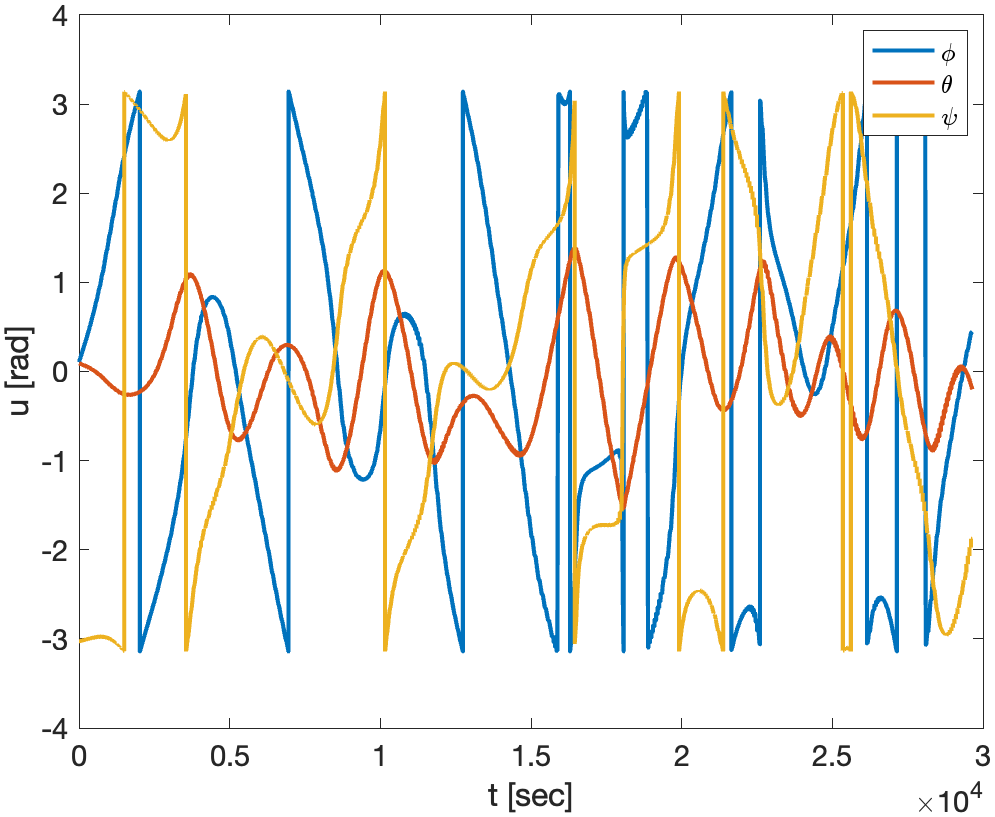
\includegraphics[width = 12cm]{Images/PS6/attitude_error_dist.png}
    \caption{312 Euler Angle Parameterization of the Rotation Error in Presence of Disturbance Torques}
    \label{fig:attitude_error_dist}
\end{figure}

\subsection{Problem 4 - You can now start modeling the Simulink spacecraft subsystem which is what the satellite believes is happening (on-board). Initially, the sensors provide ideal measurements (no bias or noise). Just use an empty box for those. The outputs of the sensors are measurements which are used for attitude determination. These measurements are computed from the reference truth or oracle.}

The sensors onboard the satellite that return reference vectors corresponding the location or direction of physical things in space are star trackers and magnetometers. For the sake of proving the functionality of the deterministic and statistical methods for attitude determination, it was deemed sufficient to only use star tracker measurements. 

The model shown in Figure \ref{fig:star_tracker_meas} depicts the simulated generation of star tracker measurements from a set of randomly selected ground truth unit vectors. In later test cases it will be seen that two sets of such random vectors were generated. One consists only of two ground truth vectors whereas the other consists of 10. The weights associated with these measurements are randomly generated as well, as there is no noise present in this validation stage. Once noise is present, the weights will be chosen much more carefully, especially in the presence of other sensors (e.g. magnetometers). To emulate noise, each component of the measurement vectors are perturbed by a random number ranging from -1 to 1 that is scaled by a so called "noise factor." Here, this factor is chosen to be 0.

\begin{figure}[H]
    \centering
    \captionsetup{ justification = centering }
    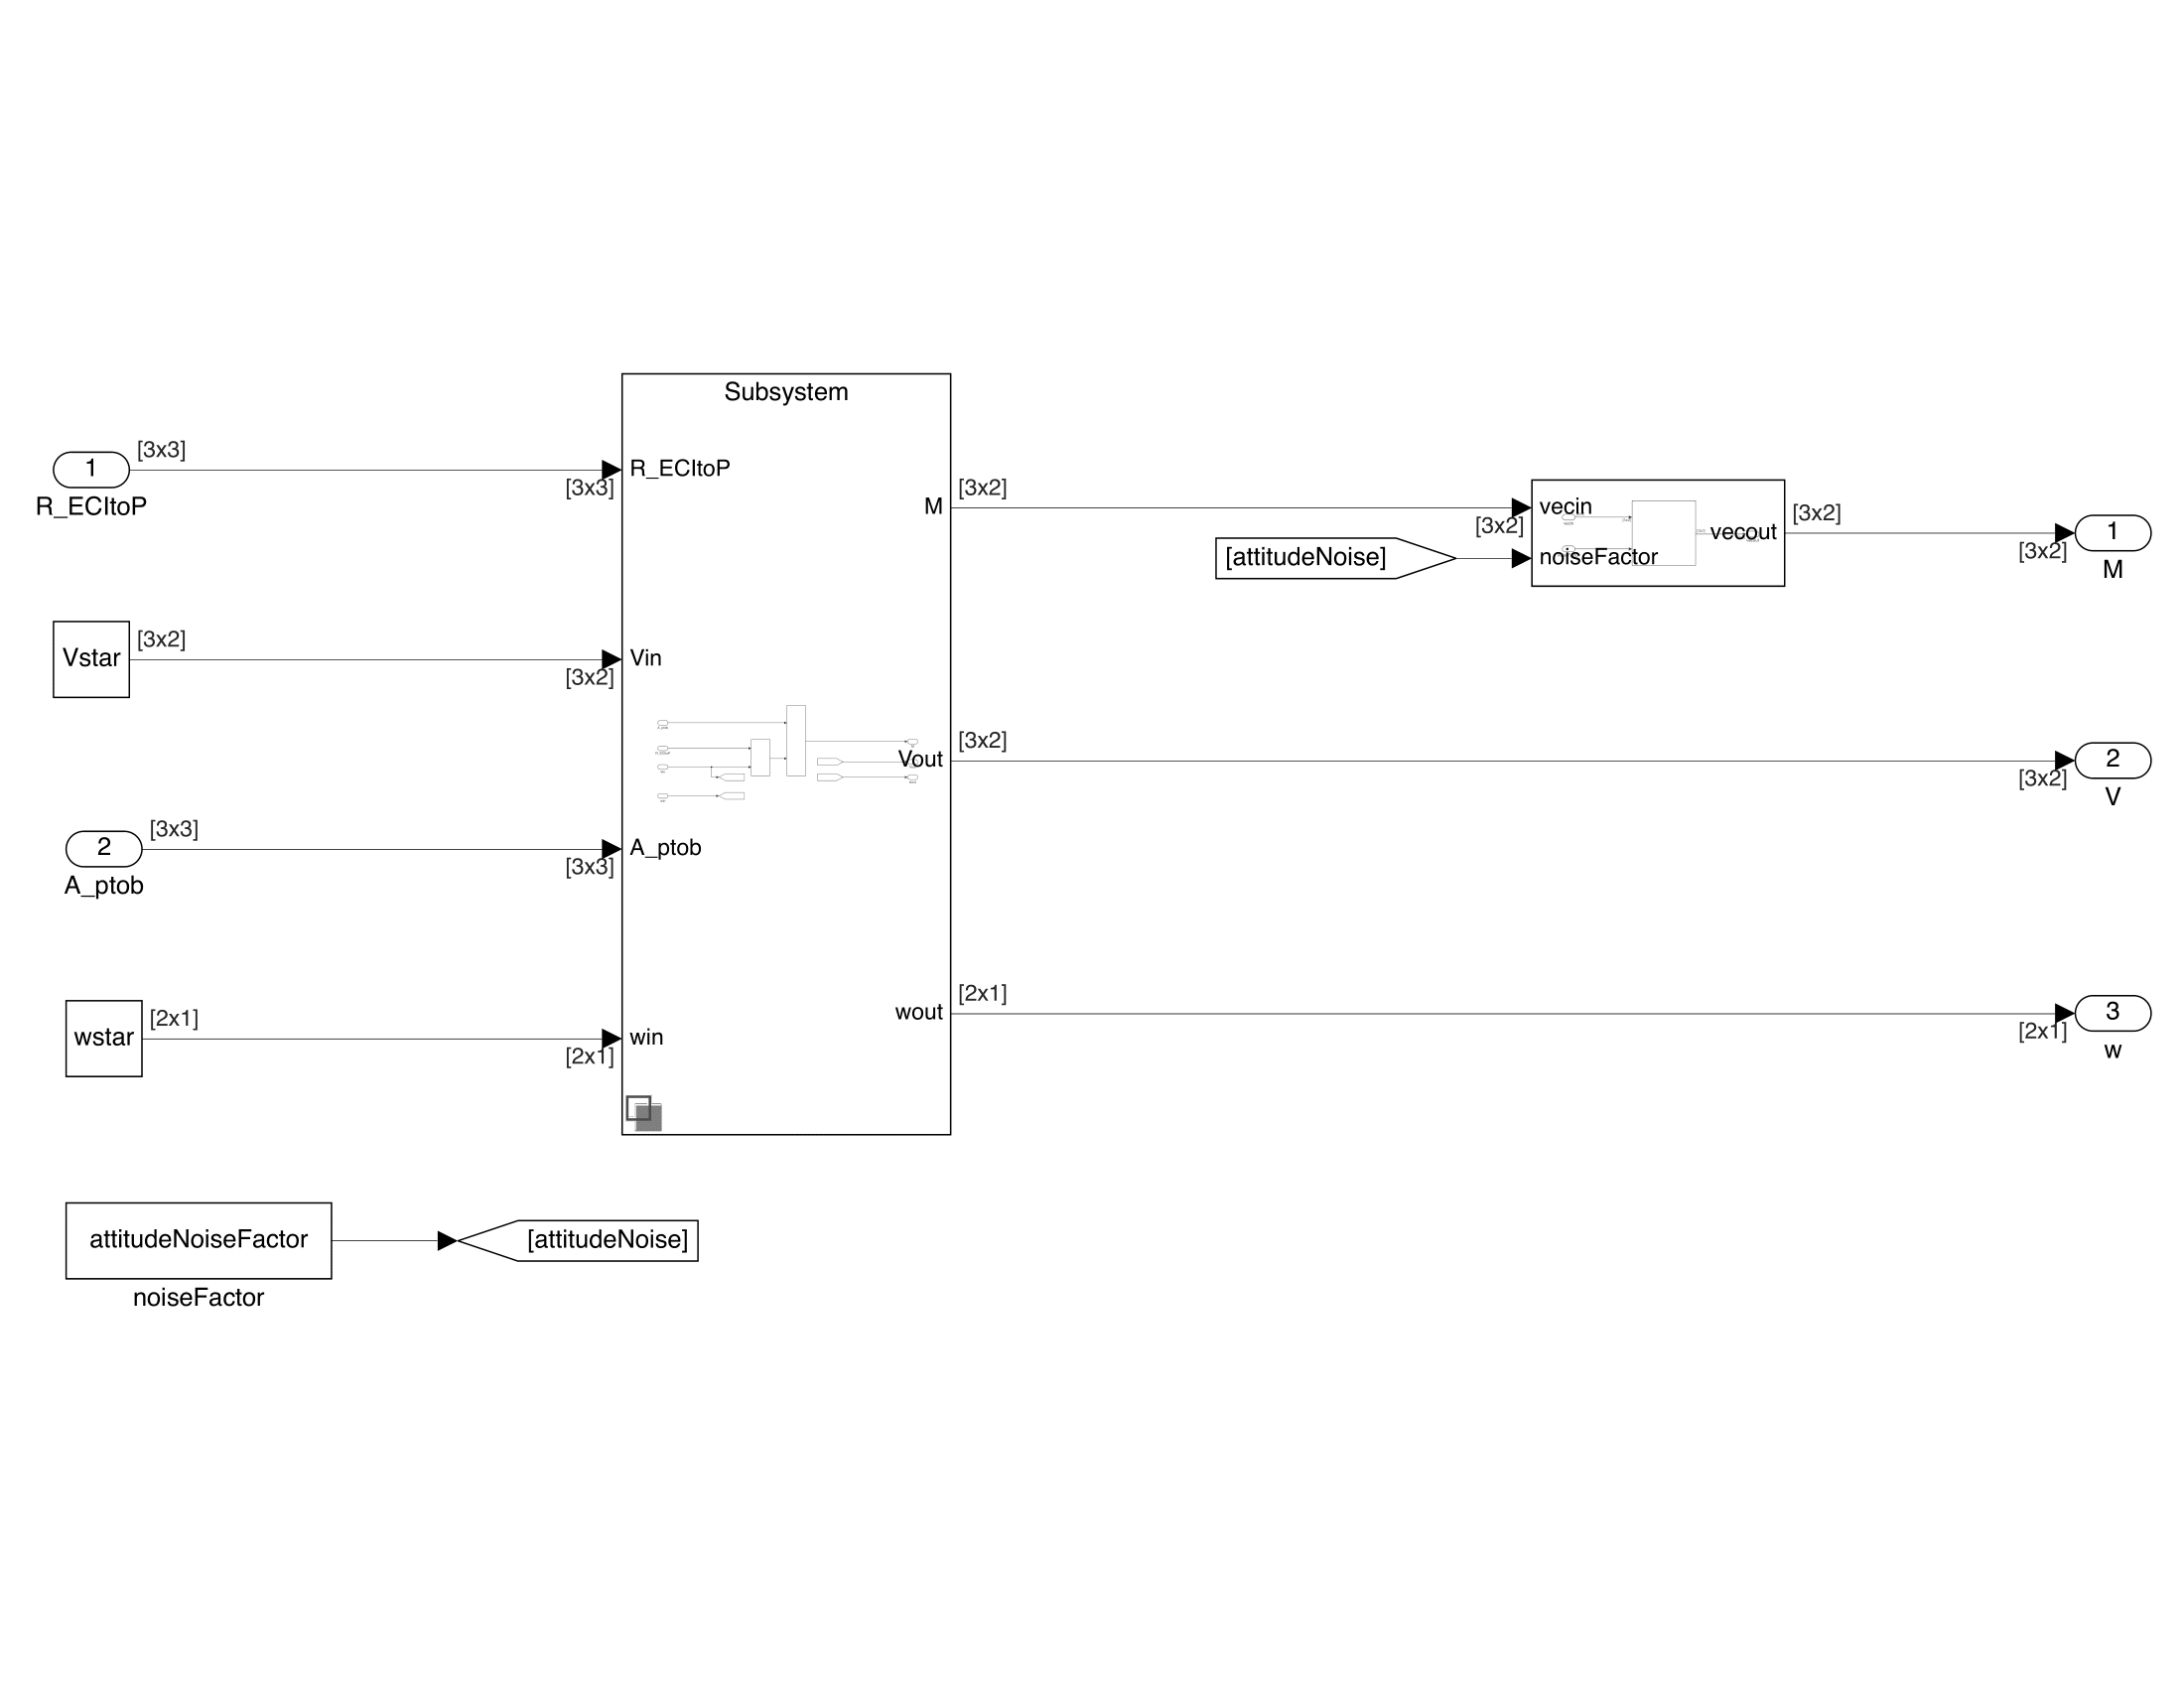
\includegraphics[trim={0.25cm 3cm 0.25cm 3cm},clip,width = 15cm]{Images/PS6/raw_meas_star.png}
    \caption{Model for Star Tracker Measurement Generation}
    \label{fig:star_tracker_meas}
\end{figure}

The model used to rotate the ground truth vectors into the body frame is seen in Figure \ref{fig:ground_truth_to_meas}.

\begin{figure}[H]
    \centering
    \captionsetup{ justification = centering }
    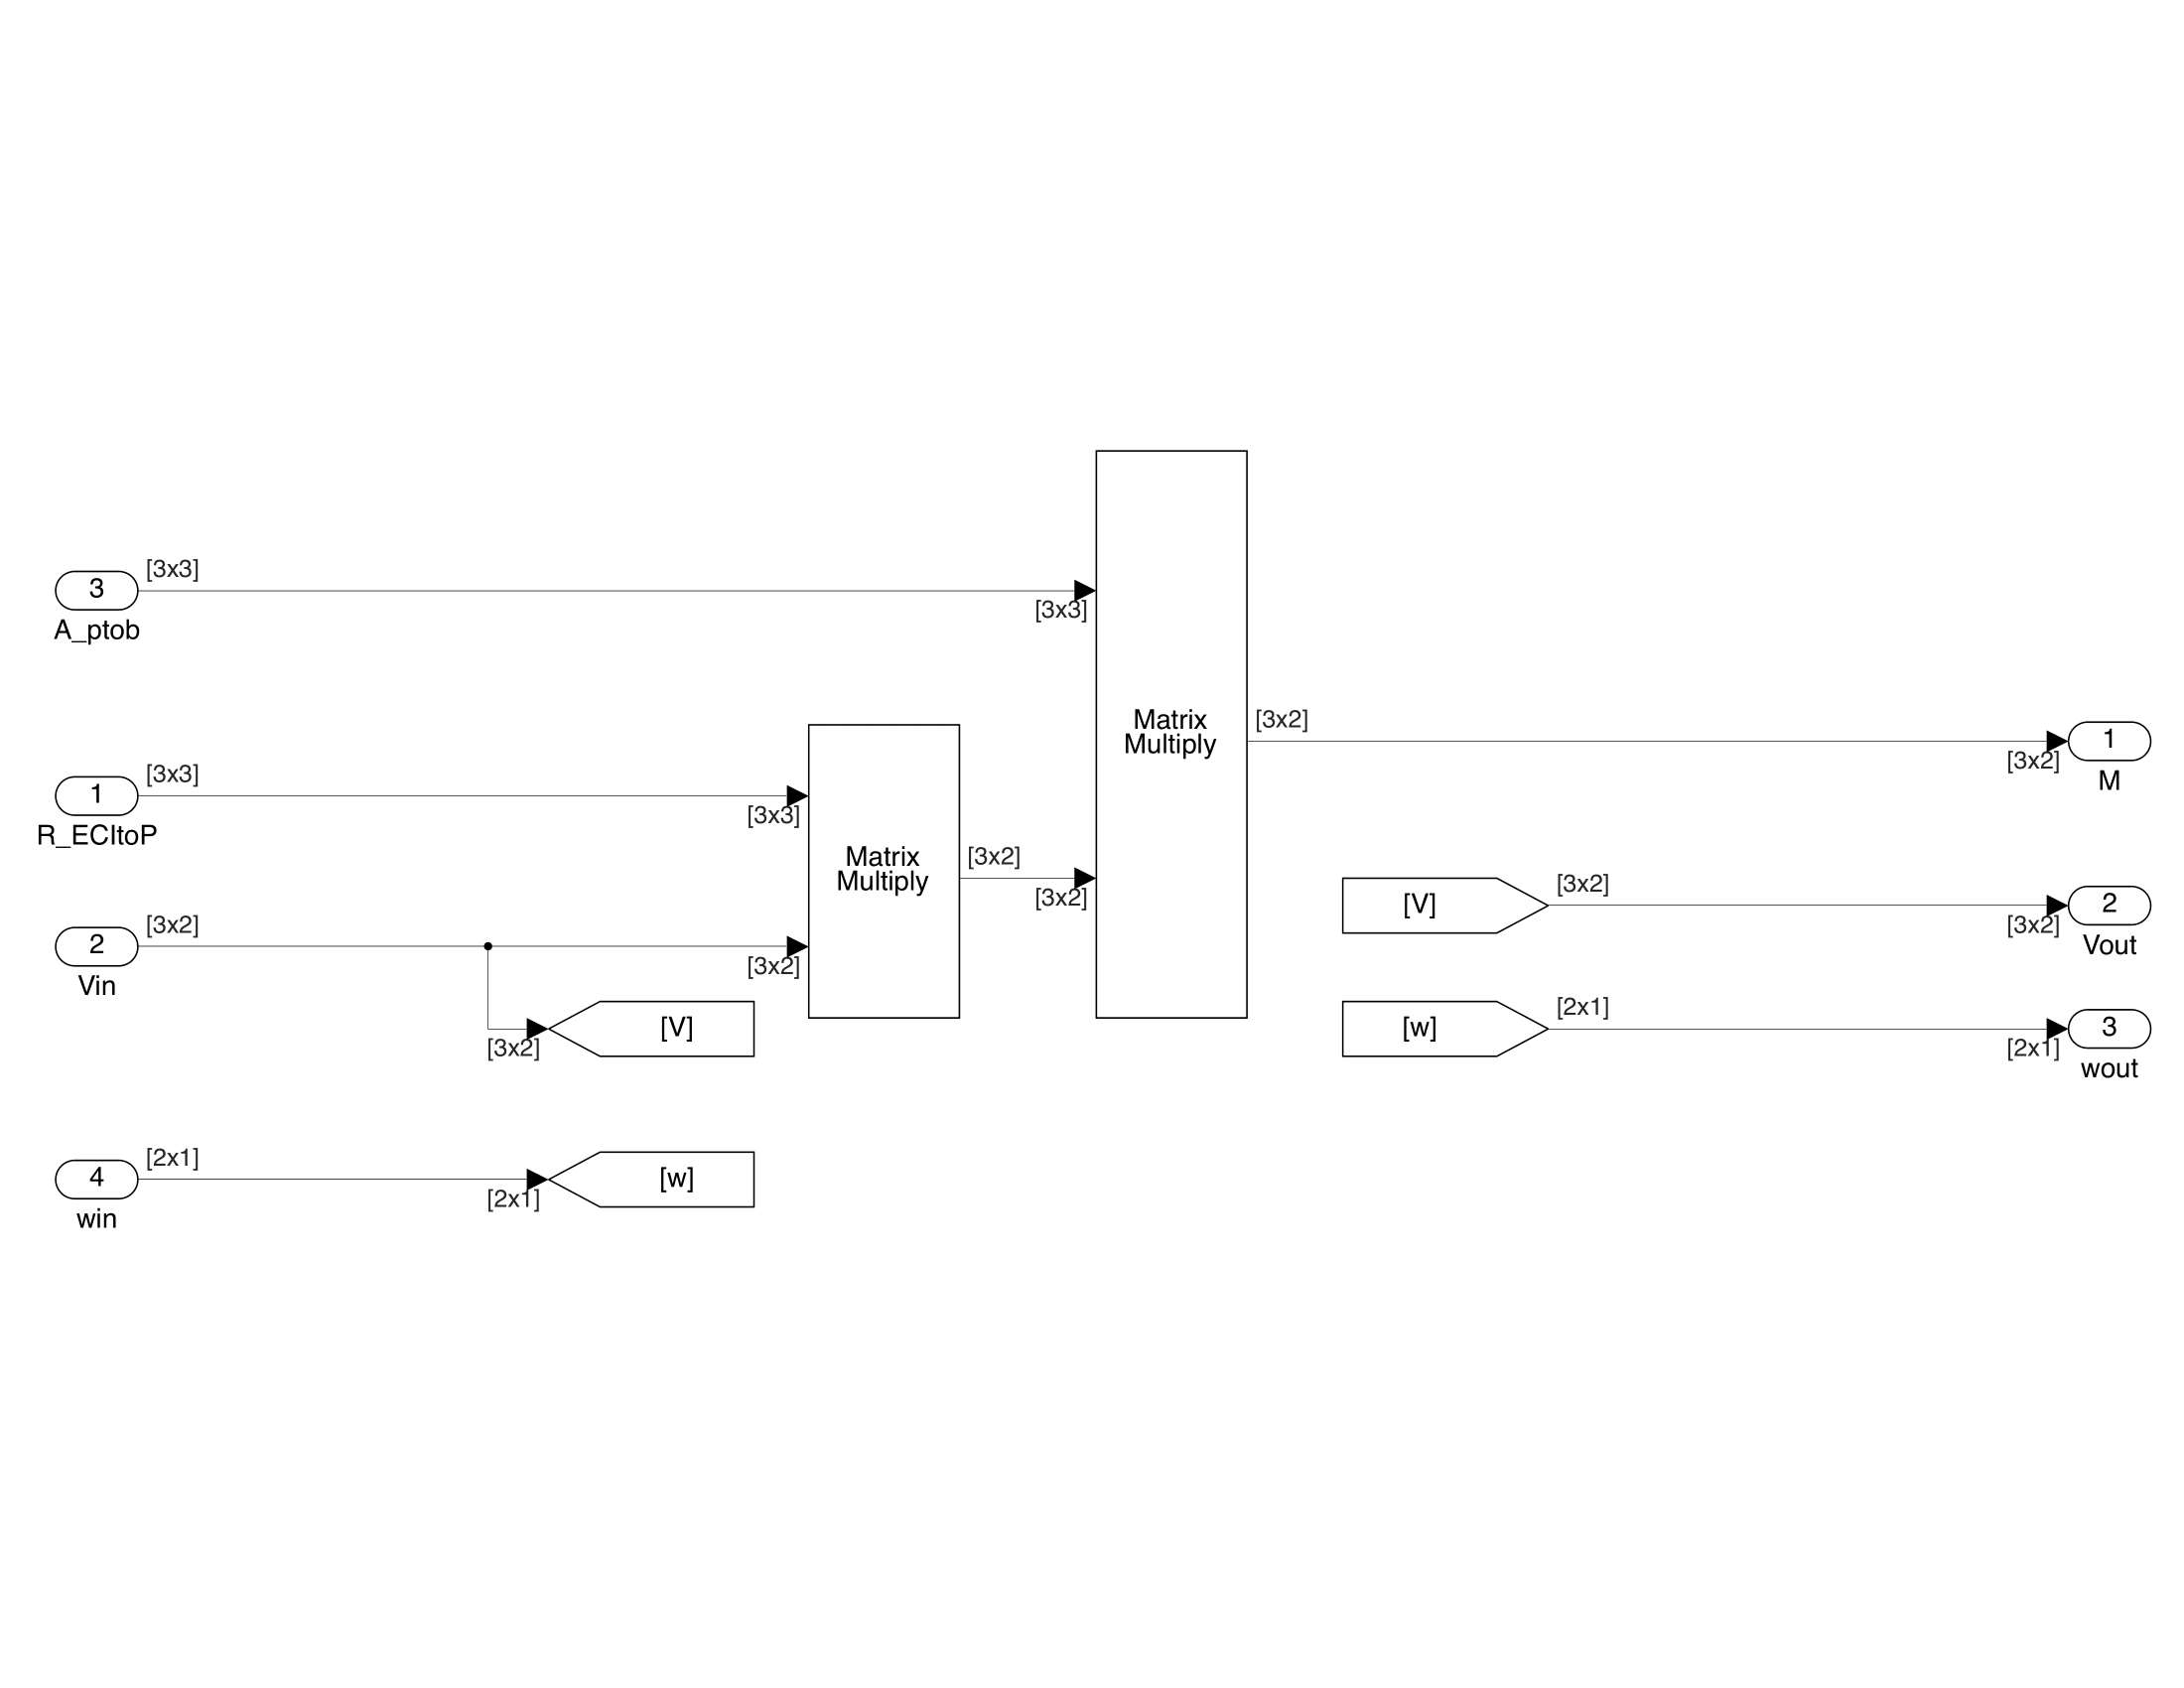
\includegraphics[trim={0.25cm 3cm 0.25cm 3cm},clip,width = 15cm]{Images/PS6/ground_truth_to_meas.png}
    \caption{Ground Truth to Measurement Model}
    \label{fig:ground_truth_to_meas}
\end{figure}

For future work, a catalog of stars would be used. Along with this, the star tracker direction in the body frame would be determined. From this, the stars that lie in the star trackers field of view would be used for the measurements while the others would be unused. This would involve allowing variable port sizes in Simulink which would pose an additional challenge.

In addition to the initialization of measurements, a system was created that would feed through sets of measurements that contain 3 or more vectors, but will create a triad if only two measurements are available. Additionally, for the case where only two measurements are available, the errors can be mitigated by creating two fictitious measurements first before generating the triad that ultimately gets fed into the deterministic determination algorithm. The feed through model can be seen in Figure \ref{fig:feedthrough_meas} whereas the fictitious measurement model can be seen in Figure \ref{fig:fictitious_meas}.

\begin{figure}[H]
    \centering
    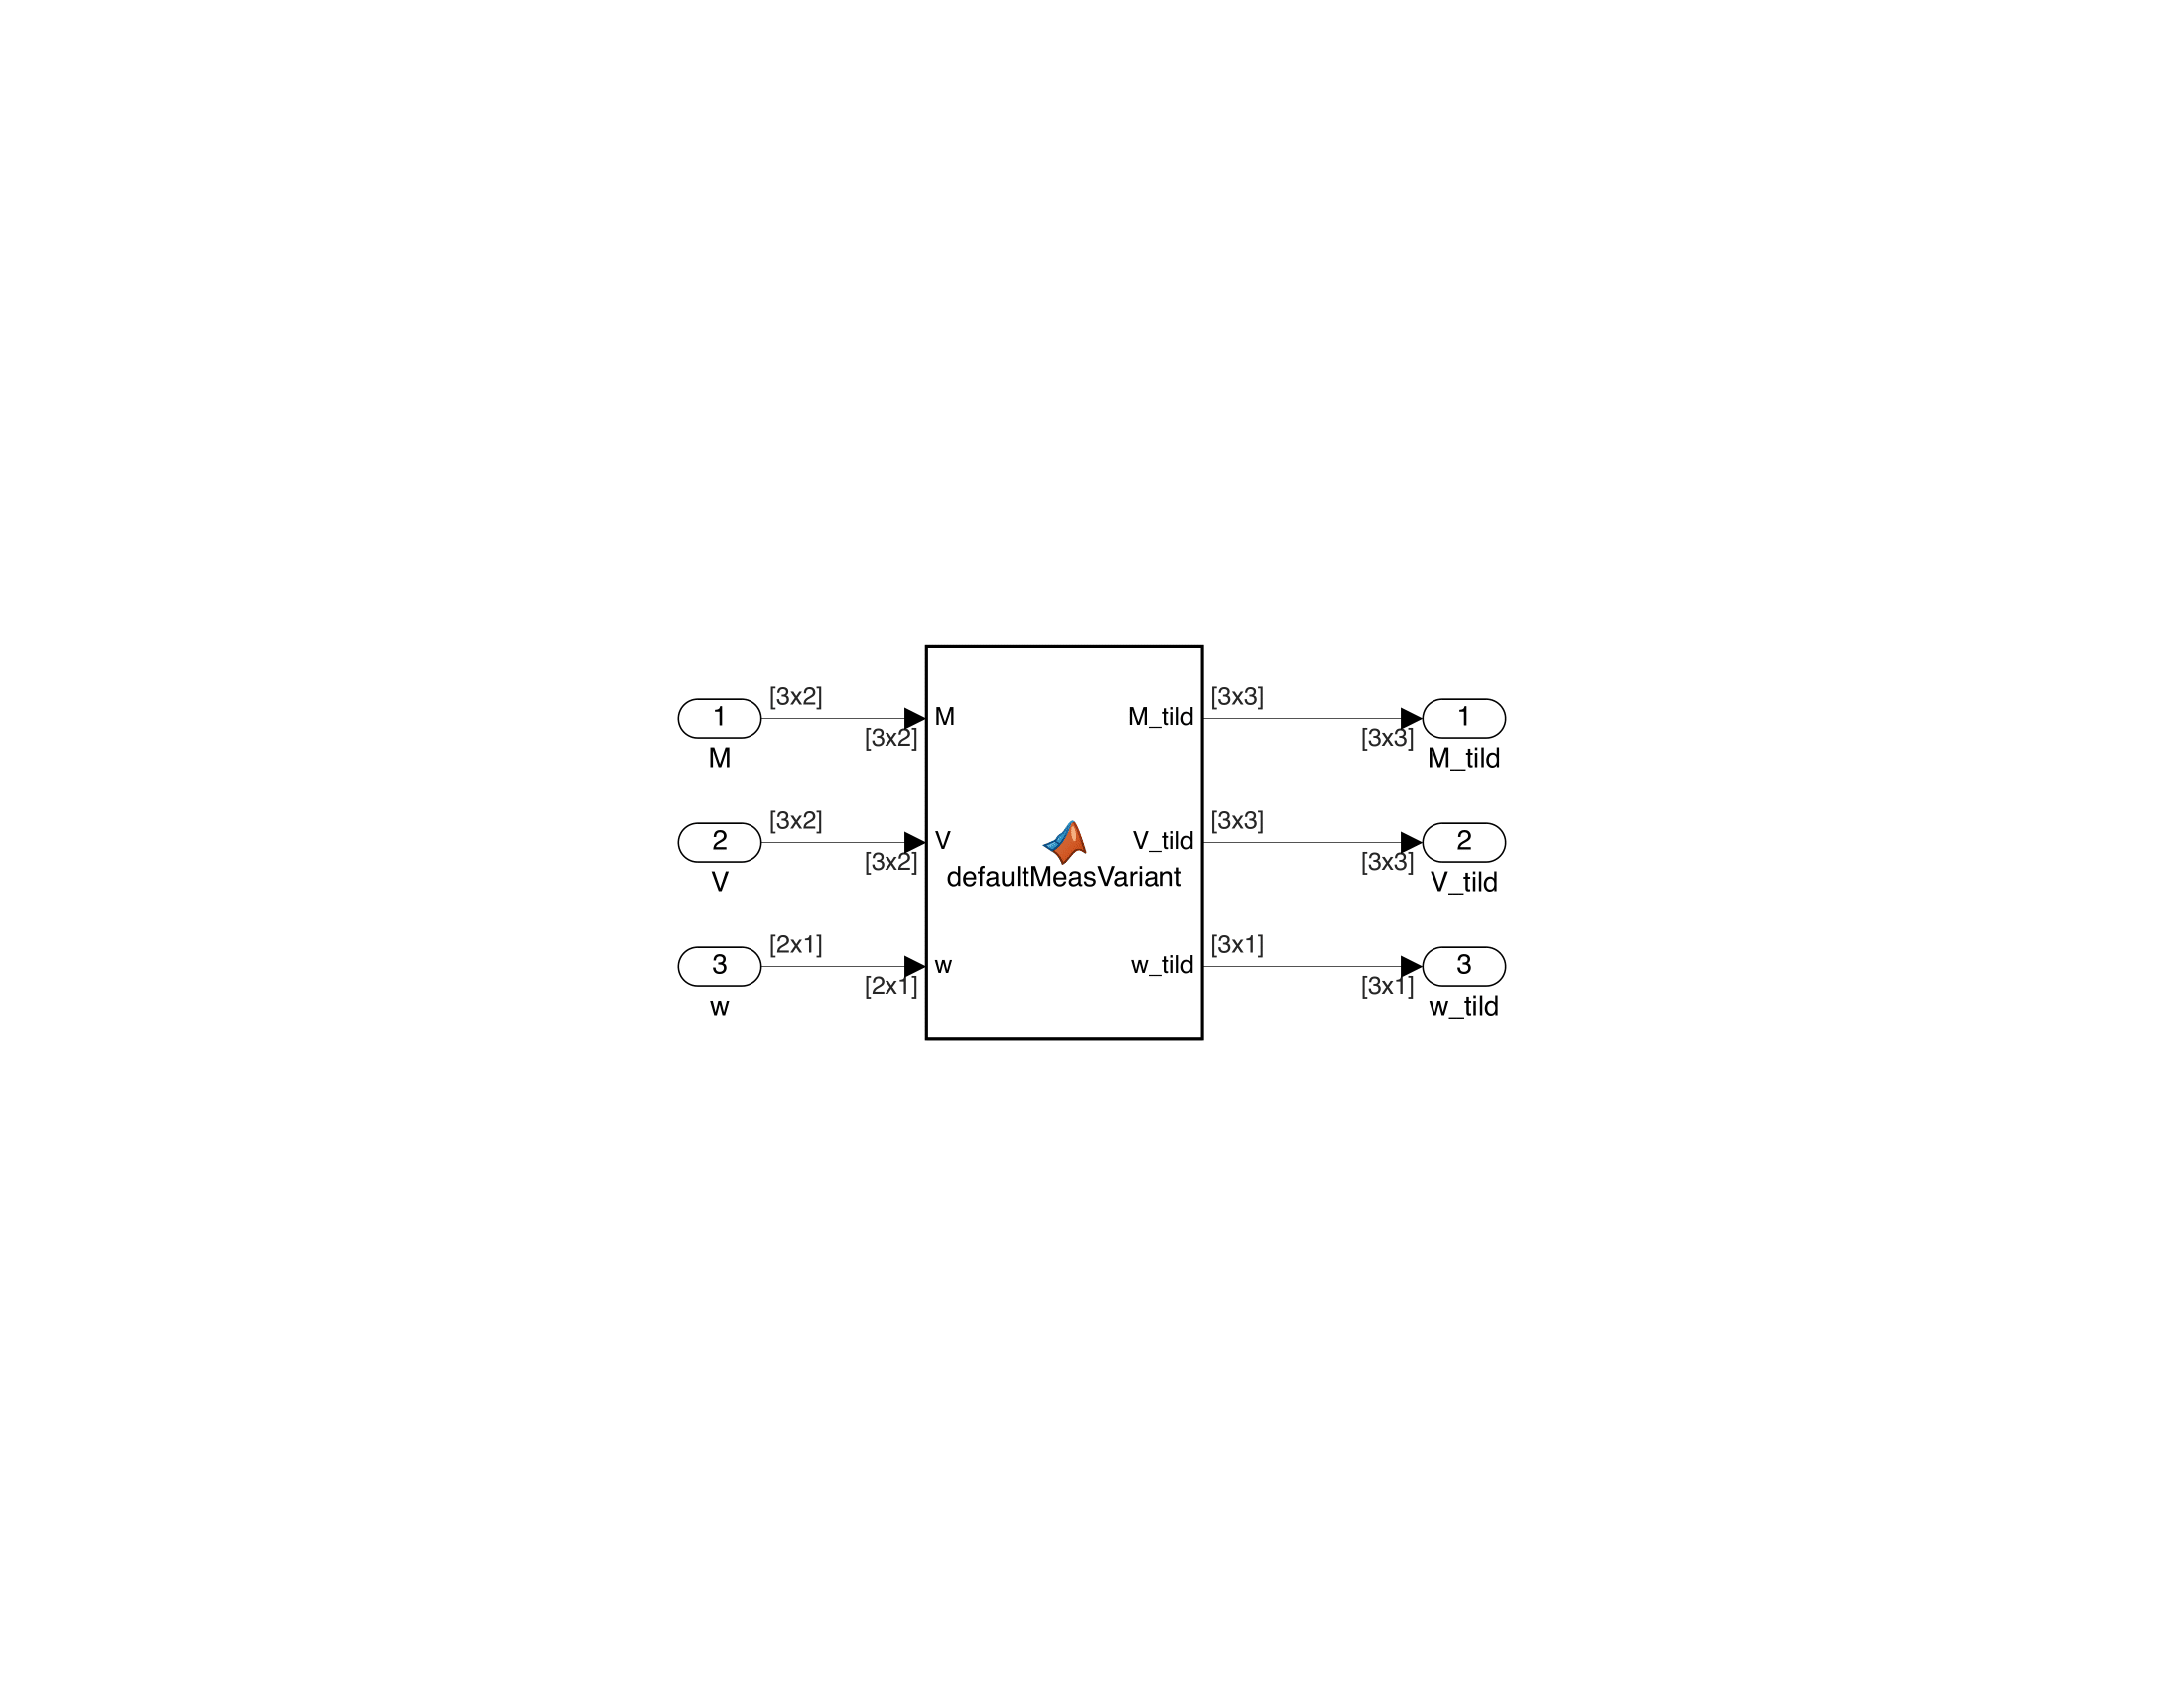
\includegraphics[trim={8cm 5cm 8cm 7cm},clip,width = 12cm]{Images/PS6/feedthrough_meas.png}
\end{figure}

\begin{figure}[H]
    \centering
    \captionsetup{ justification = centering }
    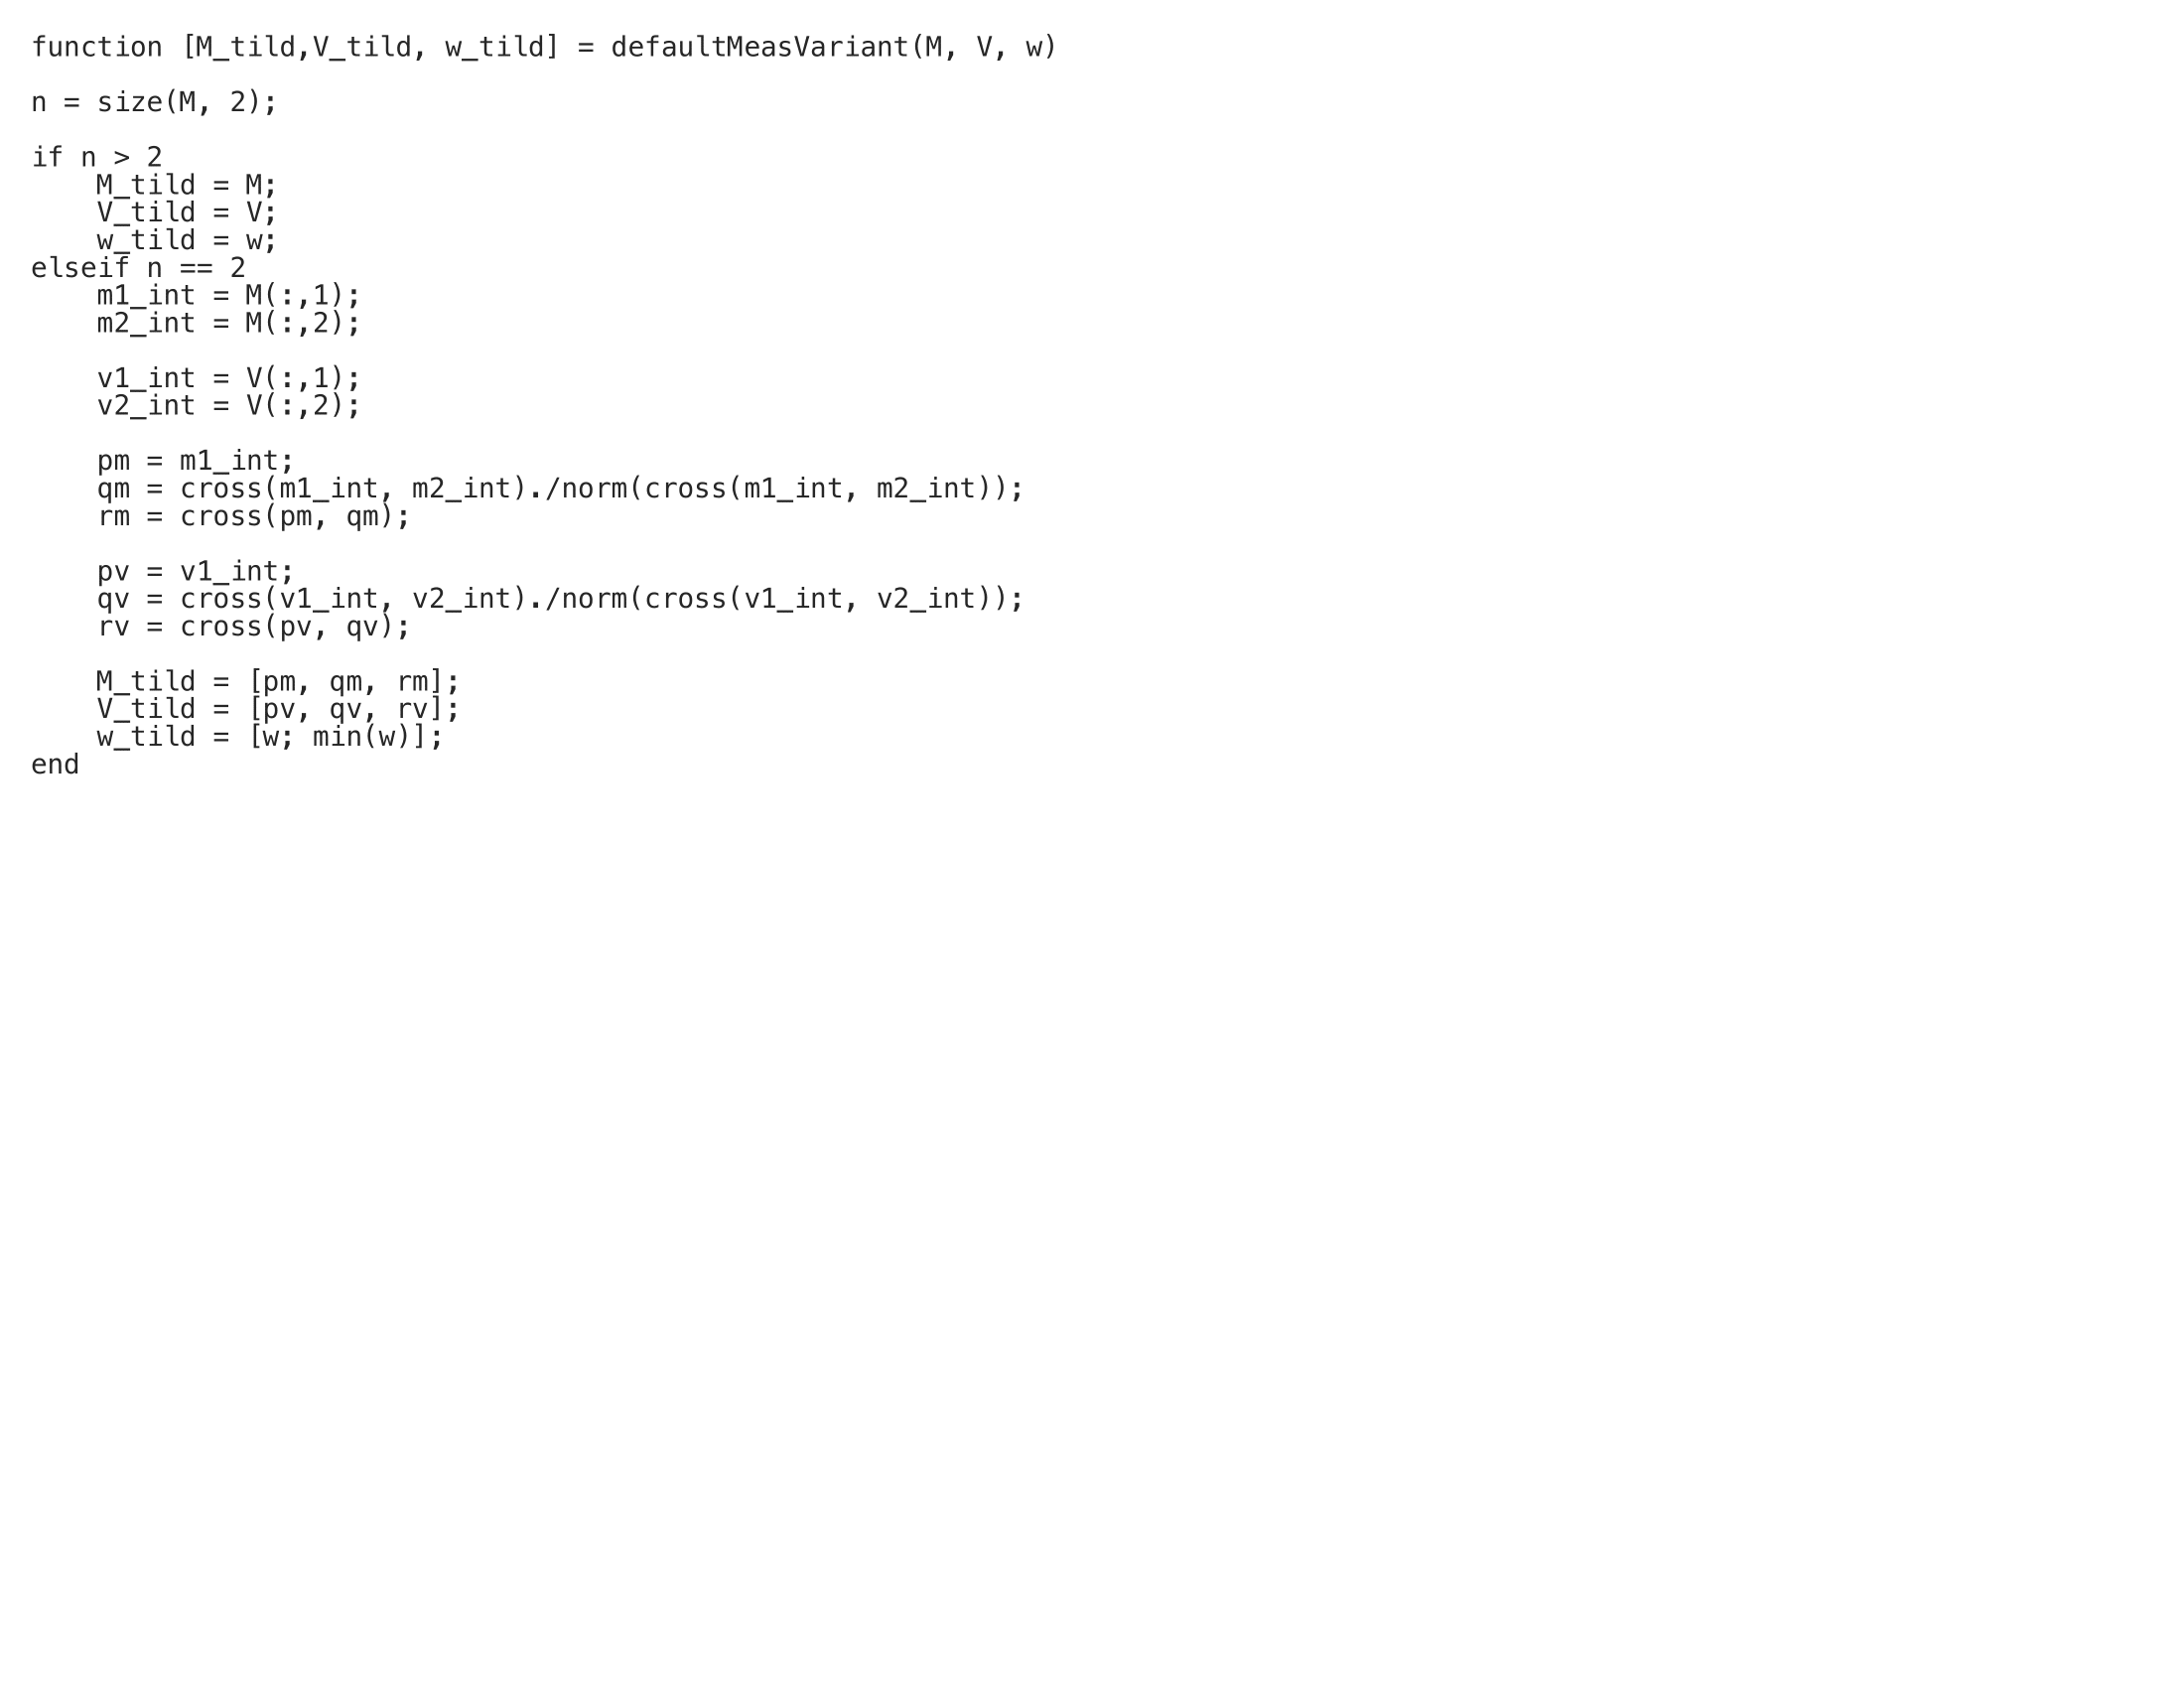
\includegraphics[trim={0cm 10cm 10cm 0cm},clip,width = 15cm]{Images/PS6/feedthrough_meas_code.png}
    \caption{Model for Star Tracker Measurement Generation}
    \label{fig:feedthrough_meas}
\end{figure}

\begin{figure}[H]
    \centering
    \captionsetup{ justification = centering }
    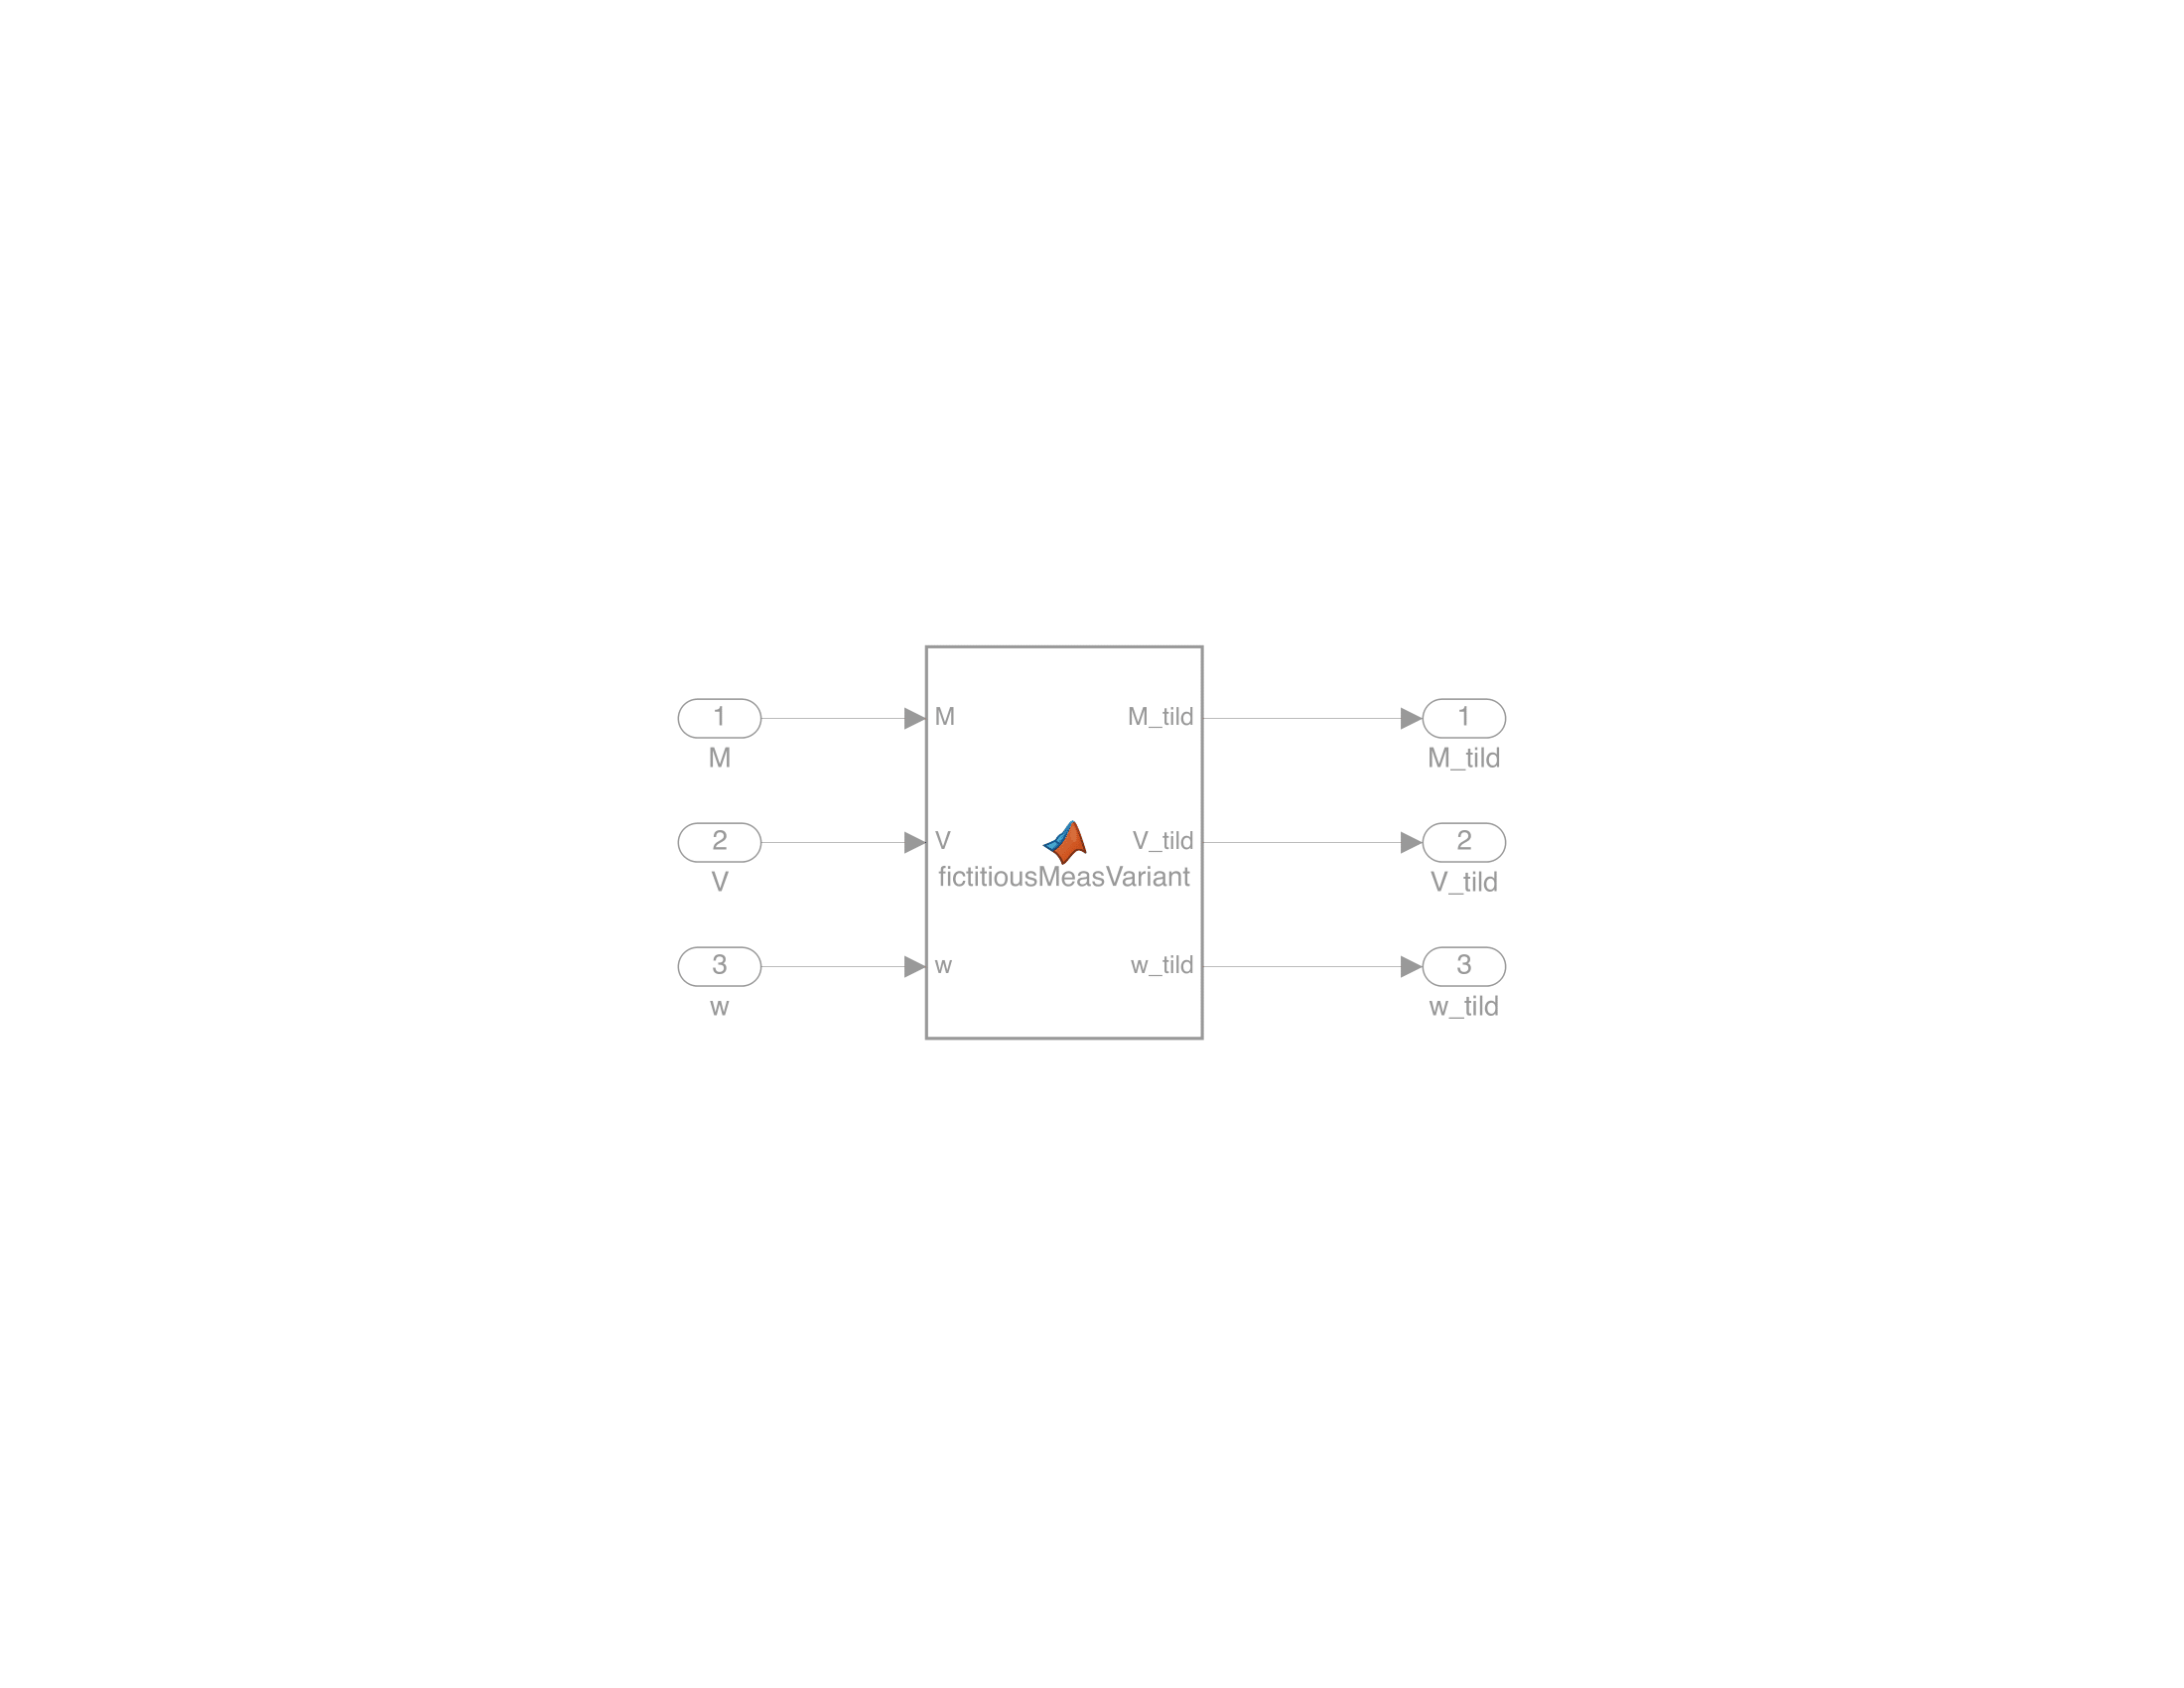
\includegraphics[trim={8cm 8cm 8cm 8cm},clip,width = 12cm]{Images/PS6/fict_meas.png}
\end{figure}

\begin{figure}[H]
    \centering
    \captionsetup{ justification = centering }
    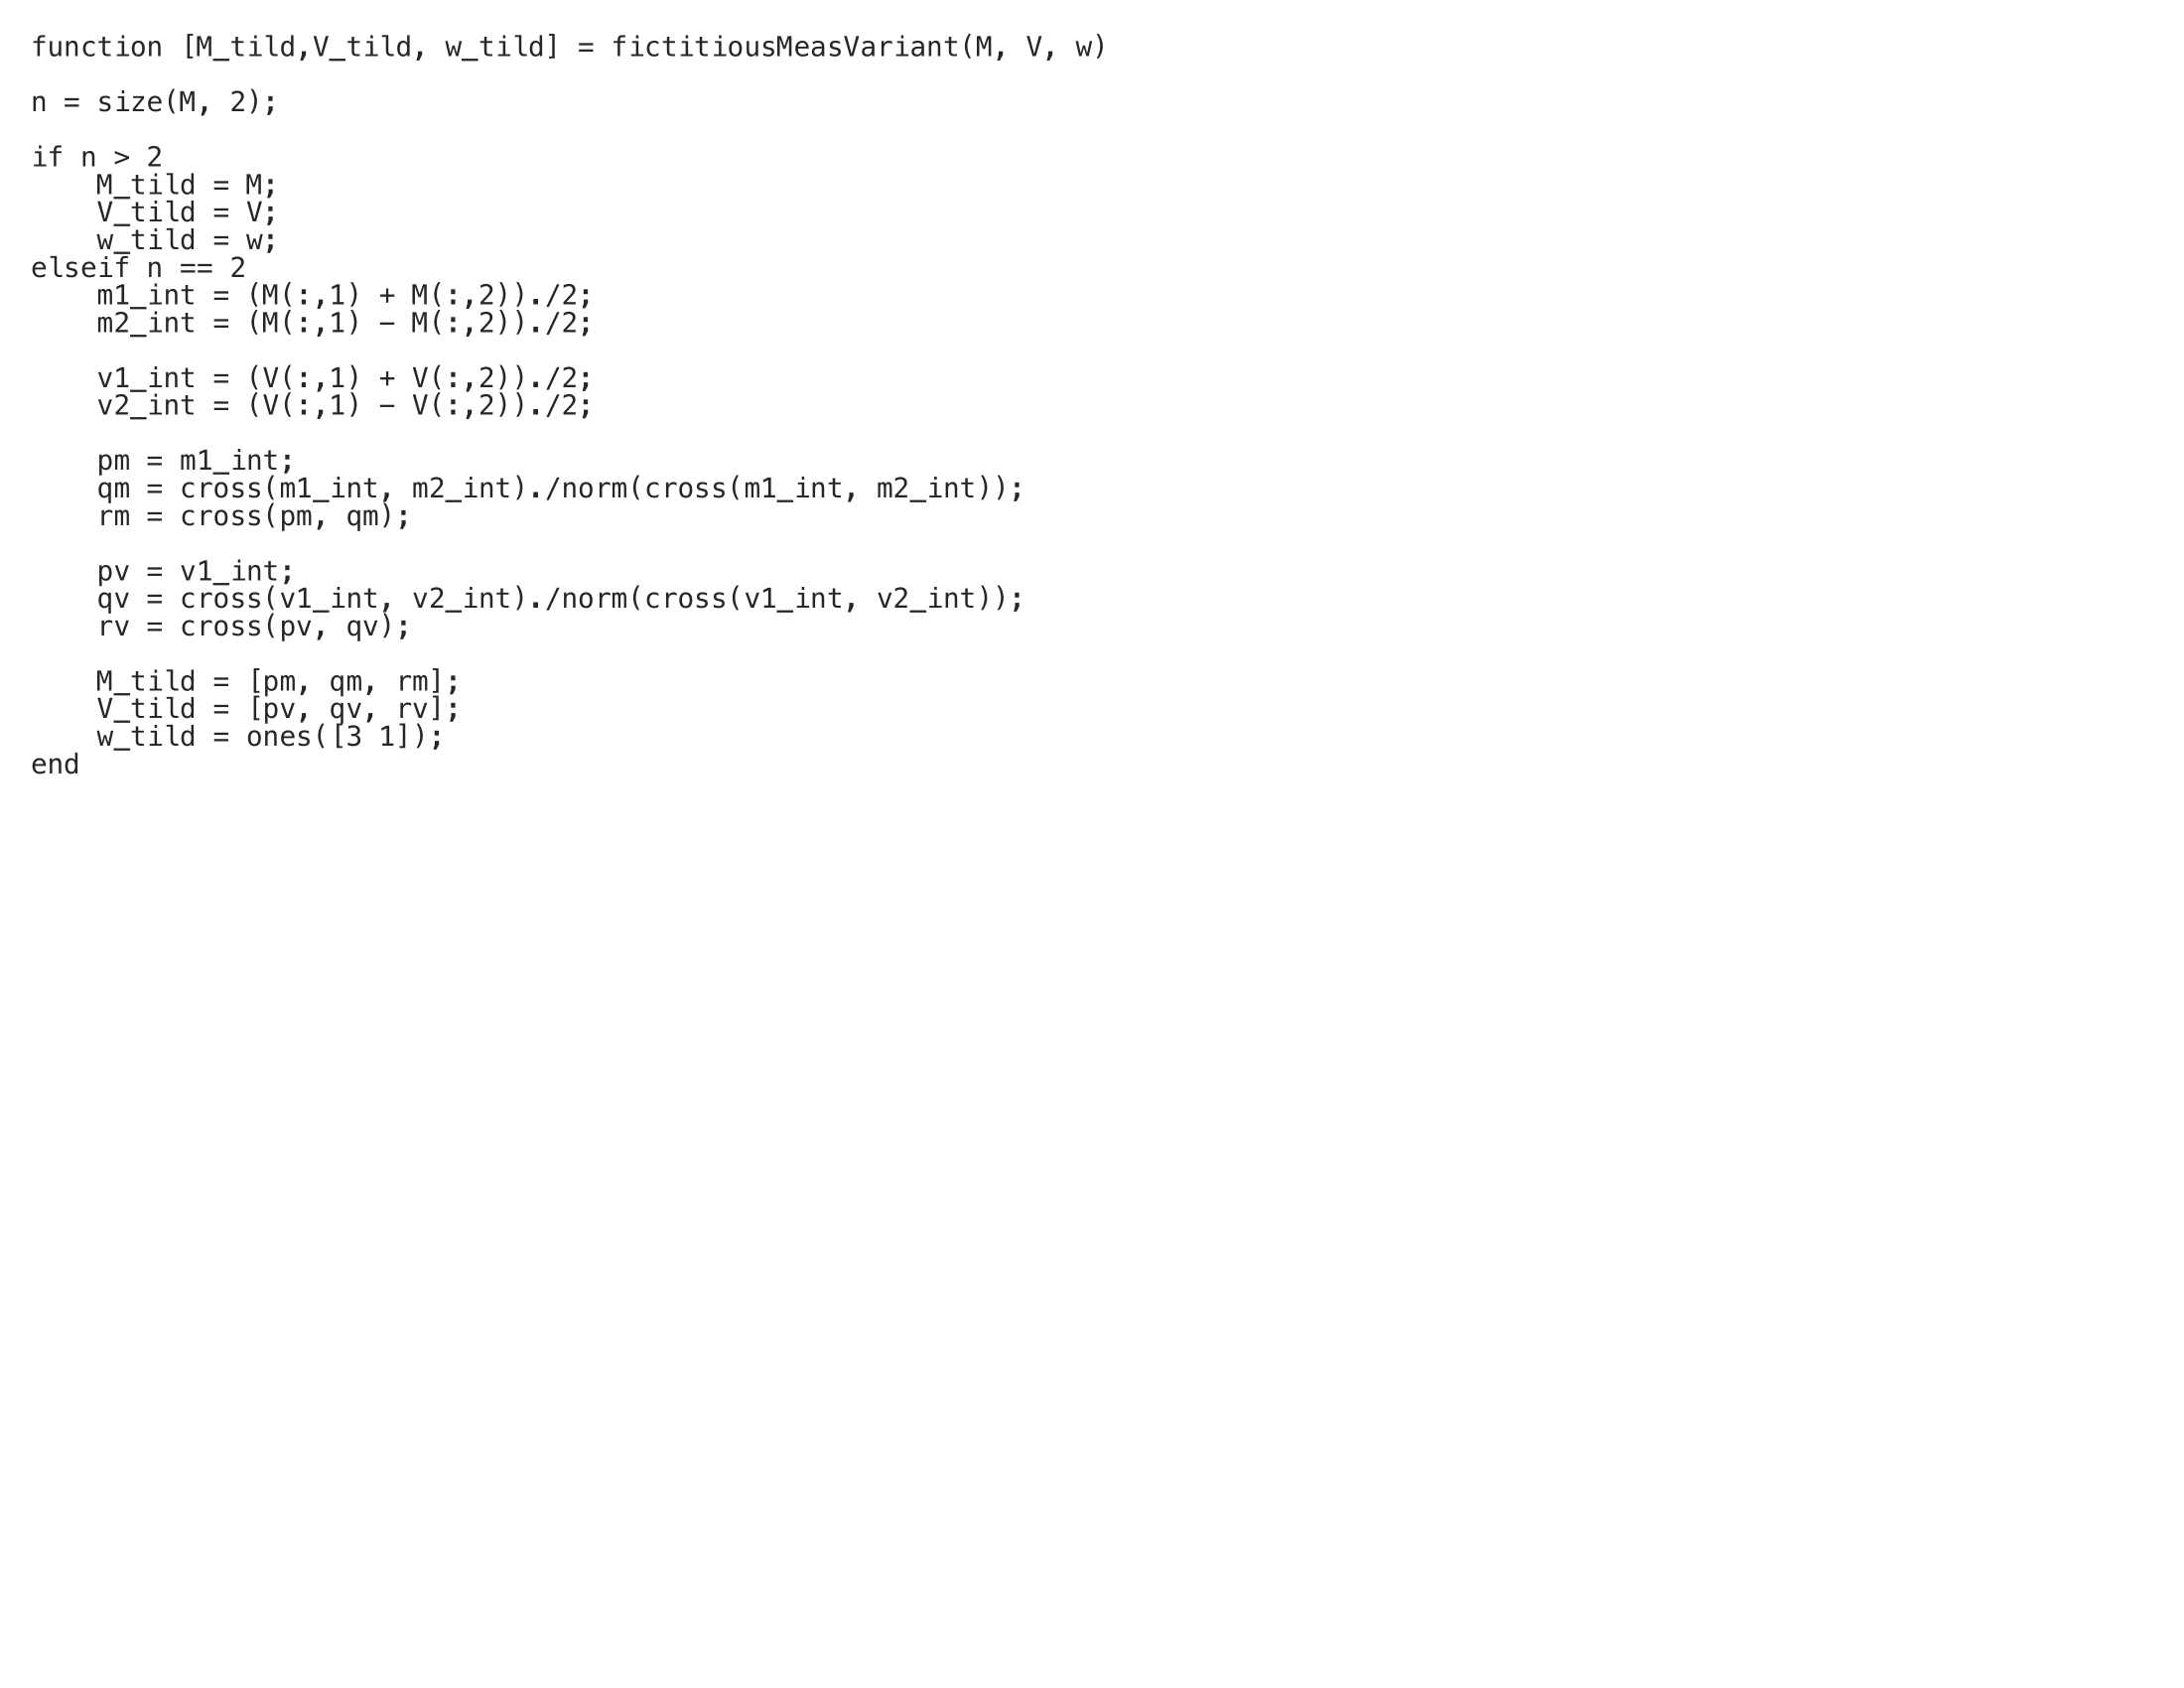
\includegraphics[trim={0cm 10cm 10cm 0cm},clip,width = 15cm]{Images/PS6/fict_meas_code.png}
    \caption{Model for Star Tracker Measurement Generation}
    \label{fig:fictitious_meas}
\end{figure}

\subsection{Problem 5 - Assume a certain set of sensors. In general, a number of unit = vectors and angular velocities can be considered as measurements.}

\subsubsection{Implement the deterministic attitude determination algorithm discussed in class and its variant which uses fictitious measurements to spread the errors across the measurements}

The deterministic attitude determination method was implemented using the model shown in Figure \ref{fig:det_attitude}.

\begin{figure}[H]
    \centering
    \captionsetup{ justification = centering }
    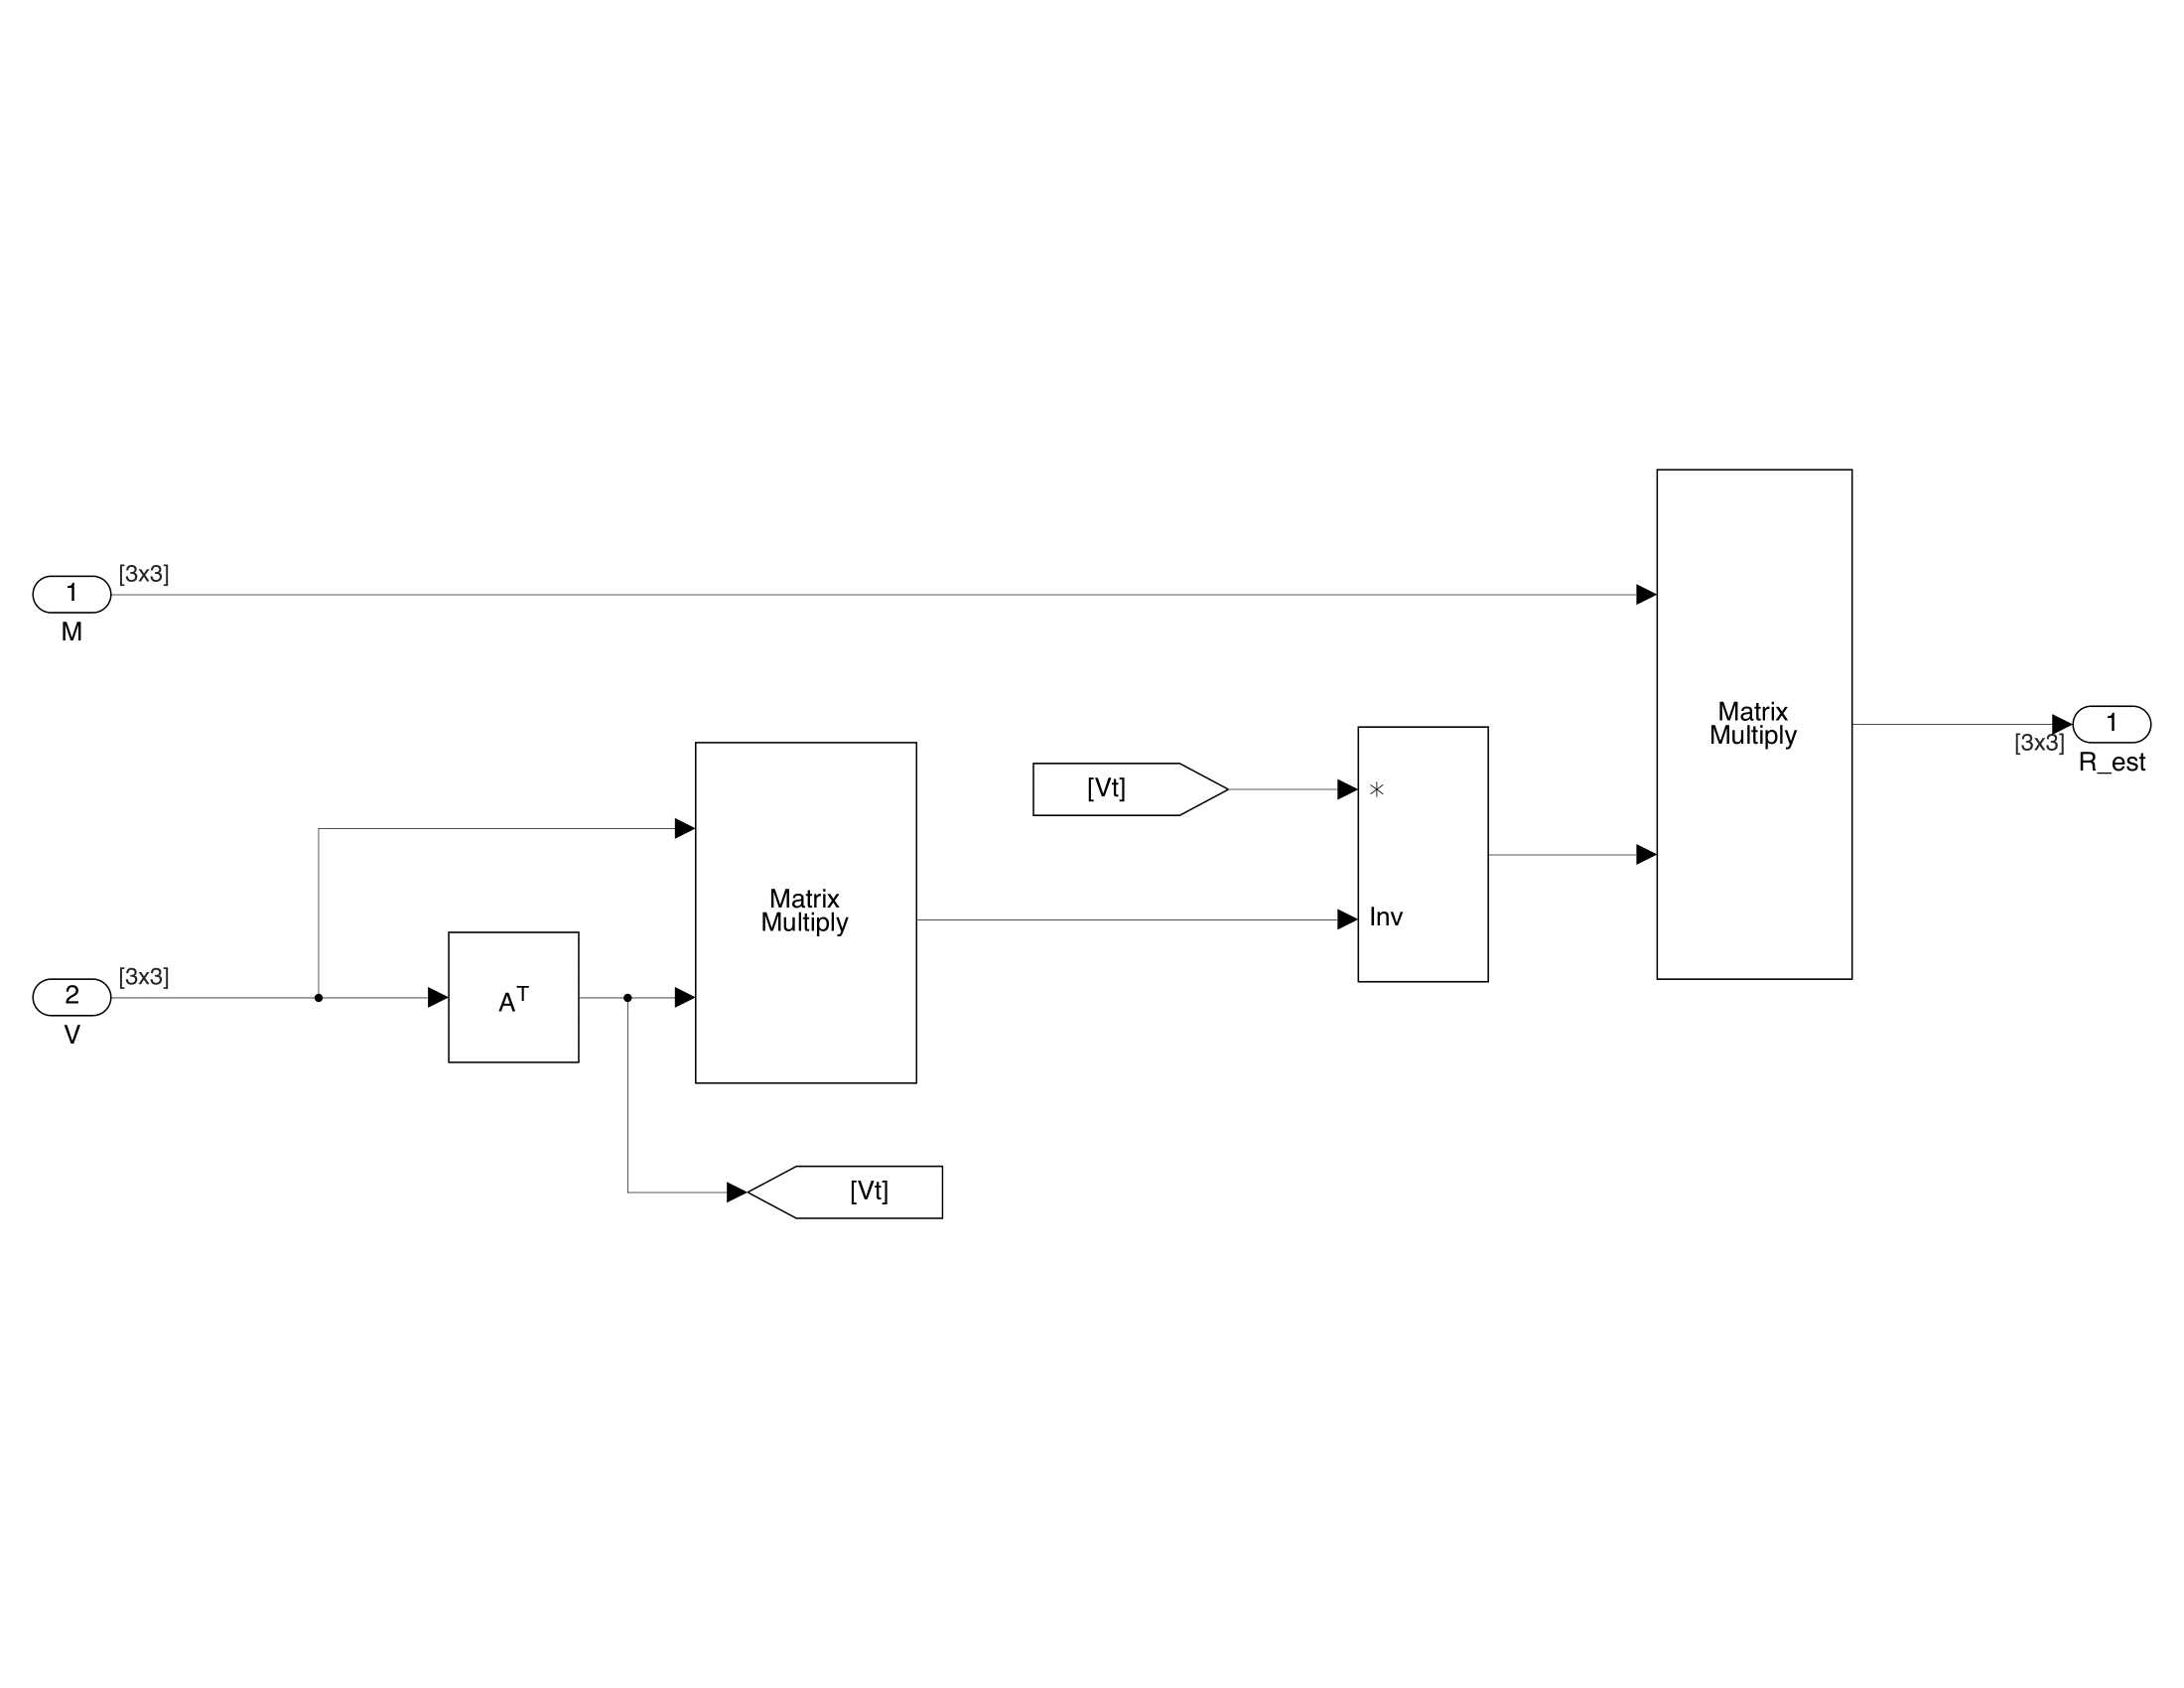
\includegraphics[trim={0.25cm 3cm 0.25cm 5cm},clip,width = 15cm]{Images/PS6/deterministicAttitude-1.png}
    \caption{Deterministic Attitude Determination Model}
    \label{fig:det_attitude}
\end{figure}

\subsubsection{Implement the statistical attitude determination algorithm discussed in class (q-method)}

The statistical attitude determination method, or the so called q-method, was implemented using the model depicted in Figure \ref{fig:stat_attitude}. 

\begin{figure}[H]
    \centering
    \captionsetup{ justification = centering }
    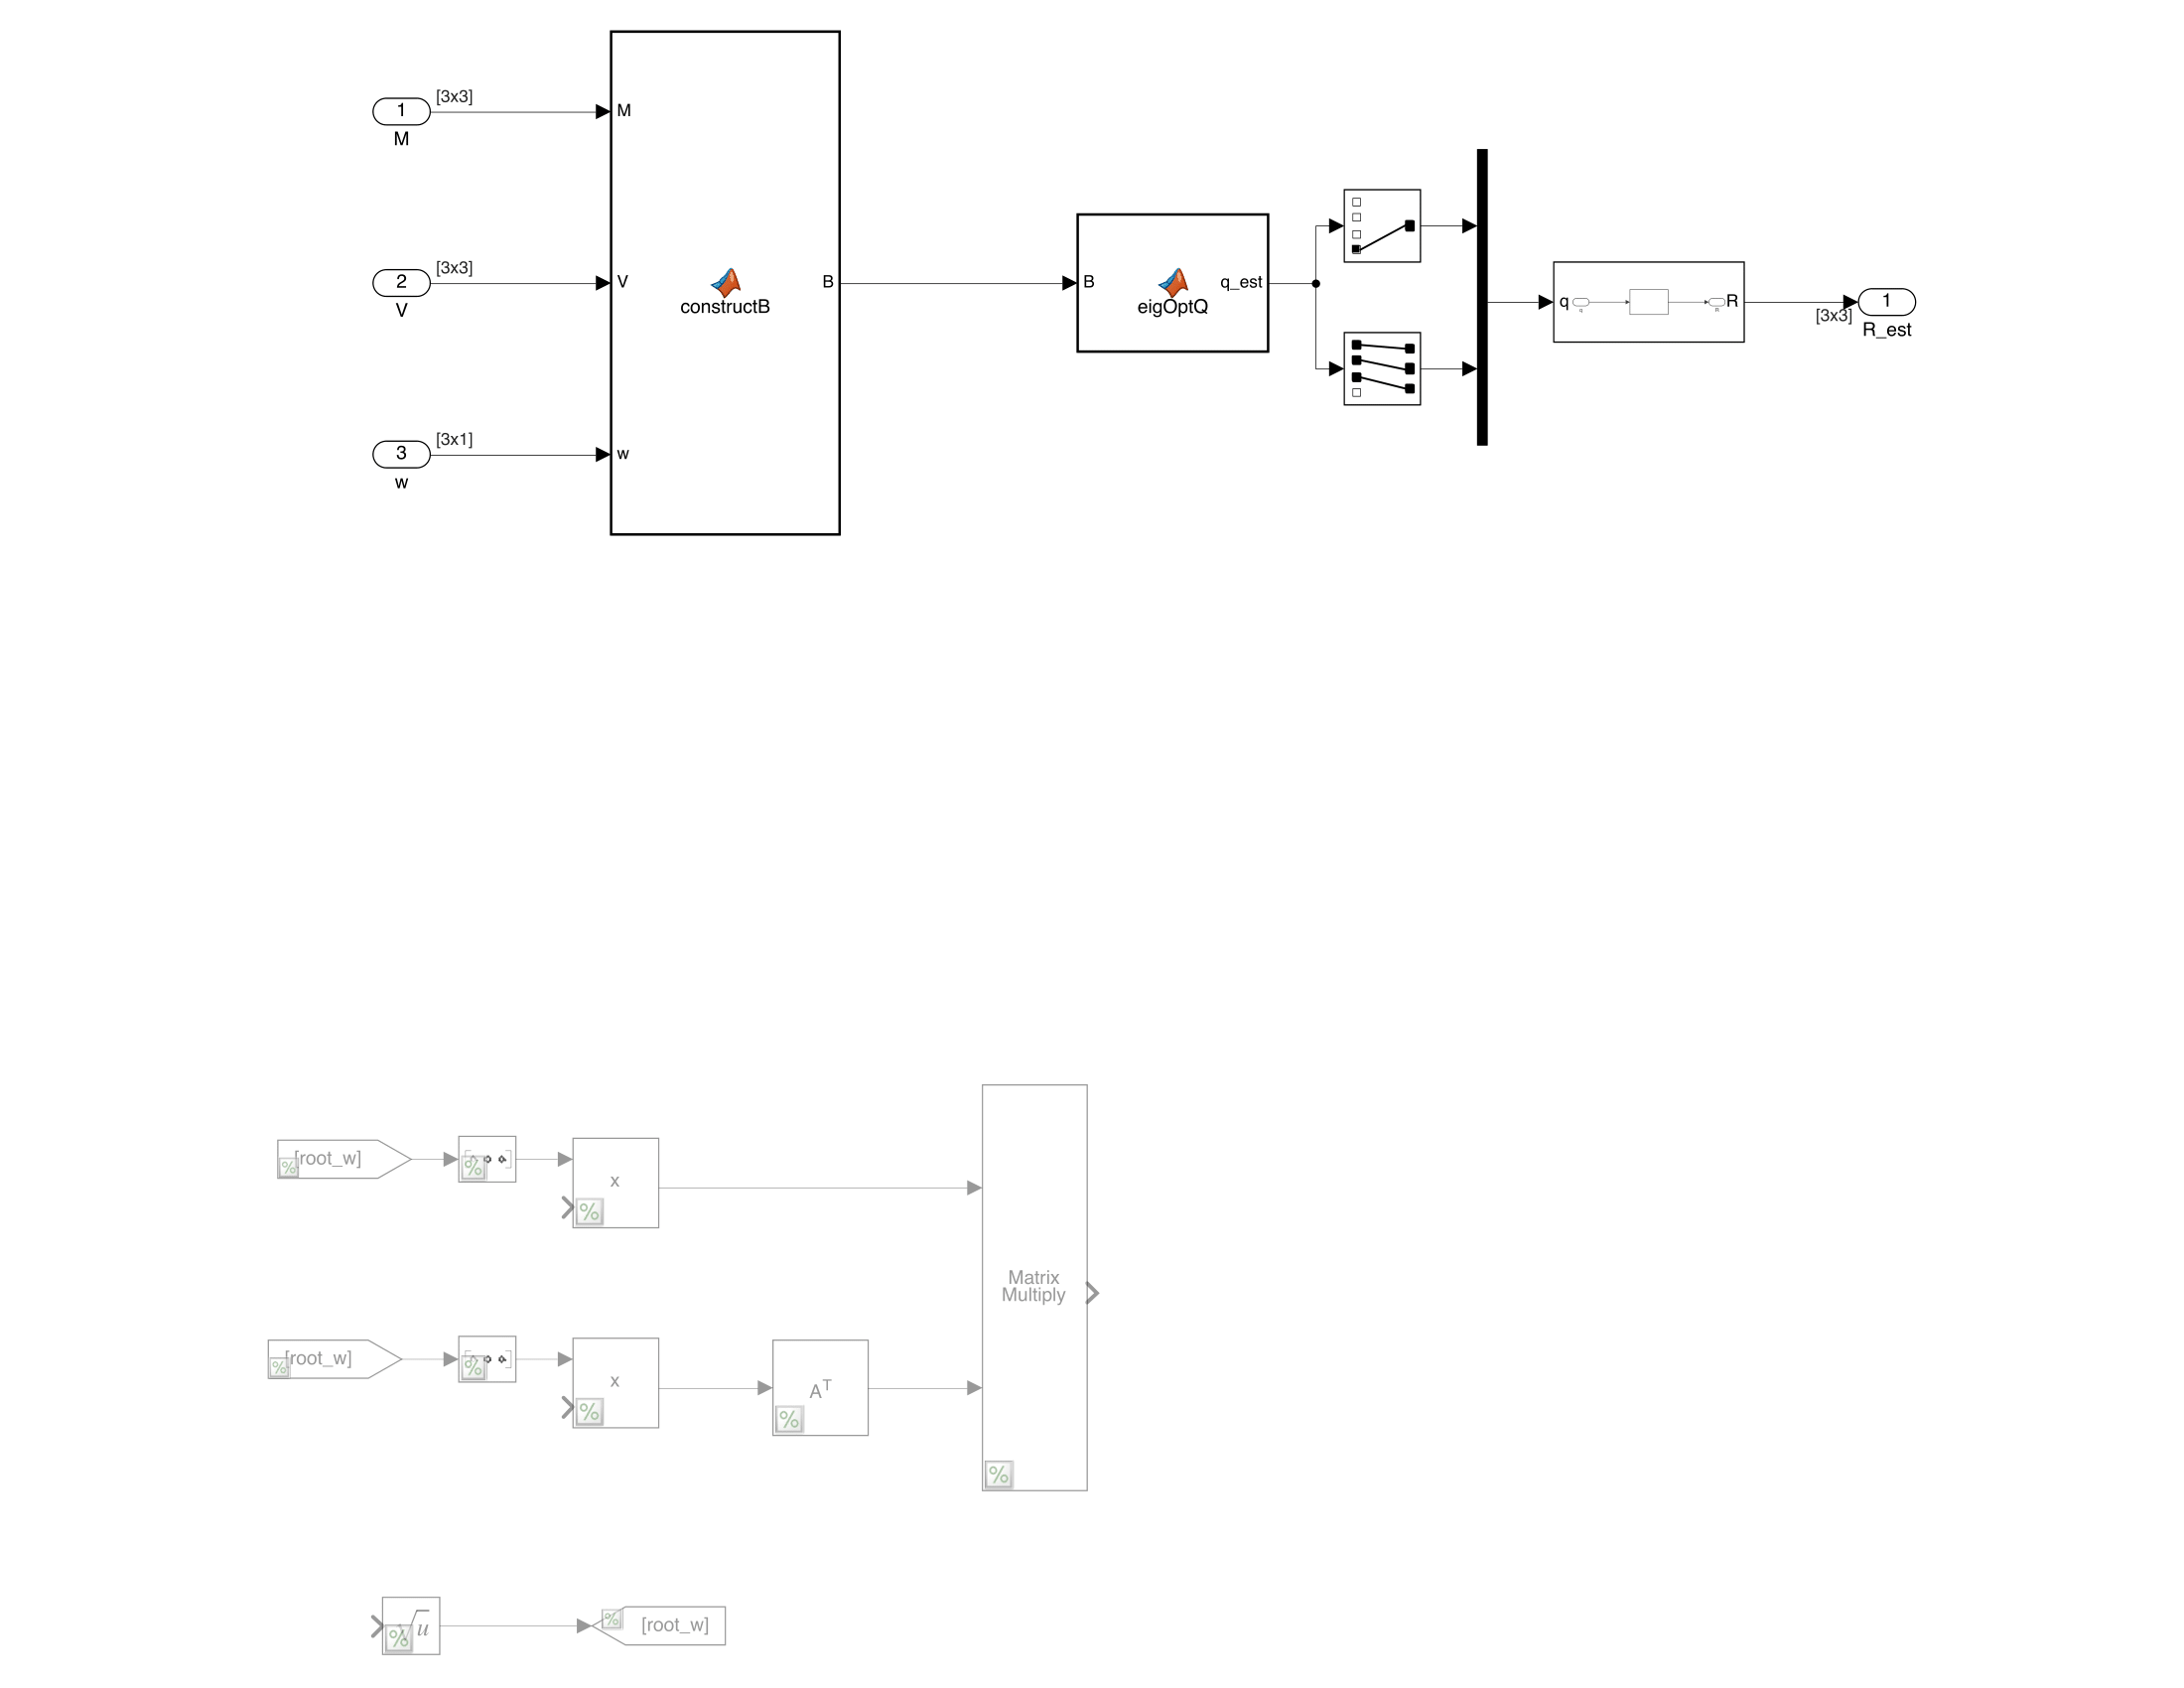
\includegraphics[trim={4cm 13cm 3cm 0cm},clip,width = 15cm]{Images/PS6/statisticalAttitude-1.png}
\end{figure}

\begin{figure}[H]
    \centering
    \captionsetup{ justification = centering }
    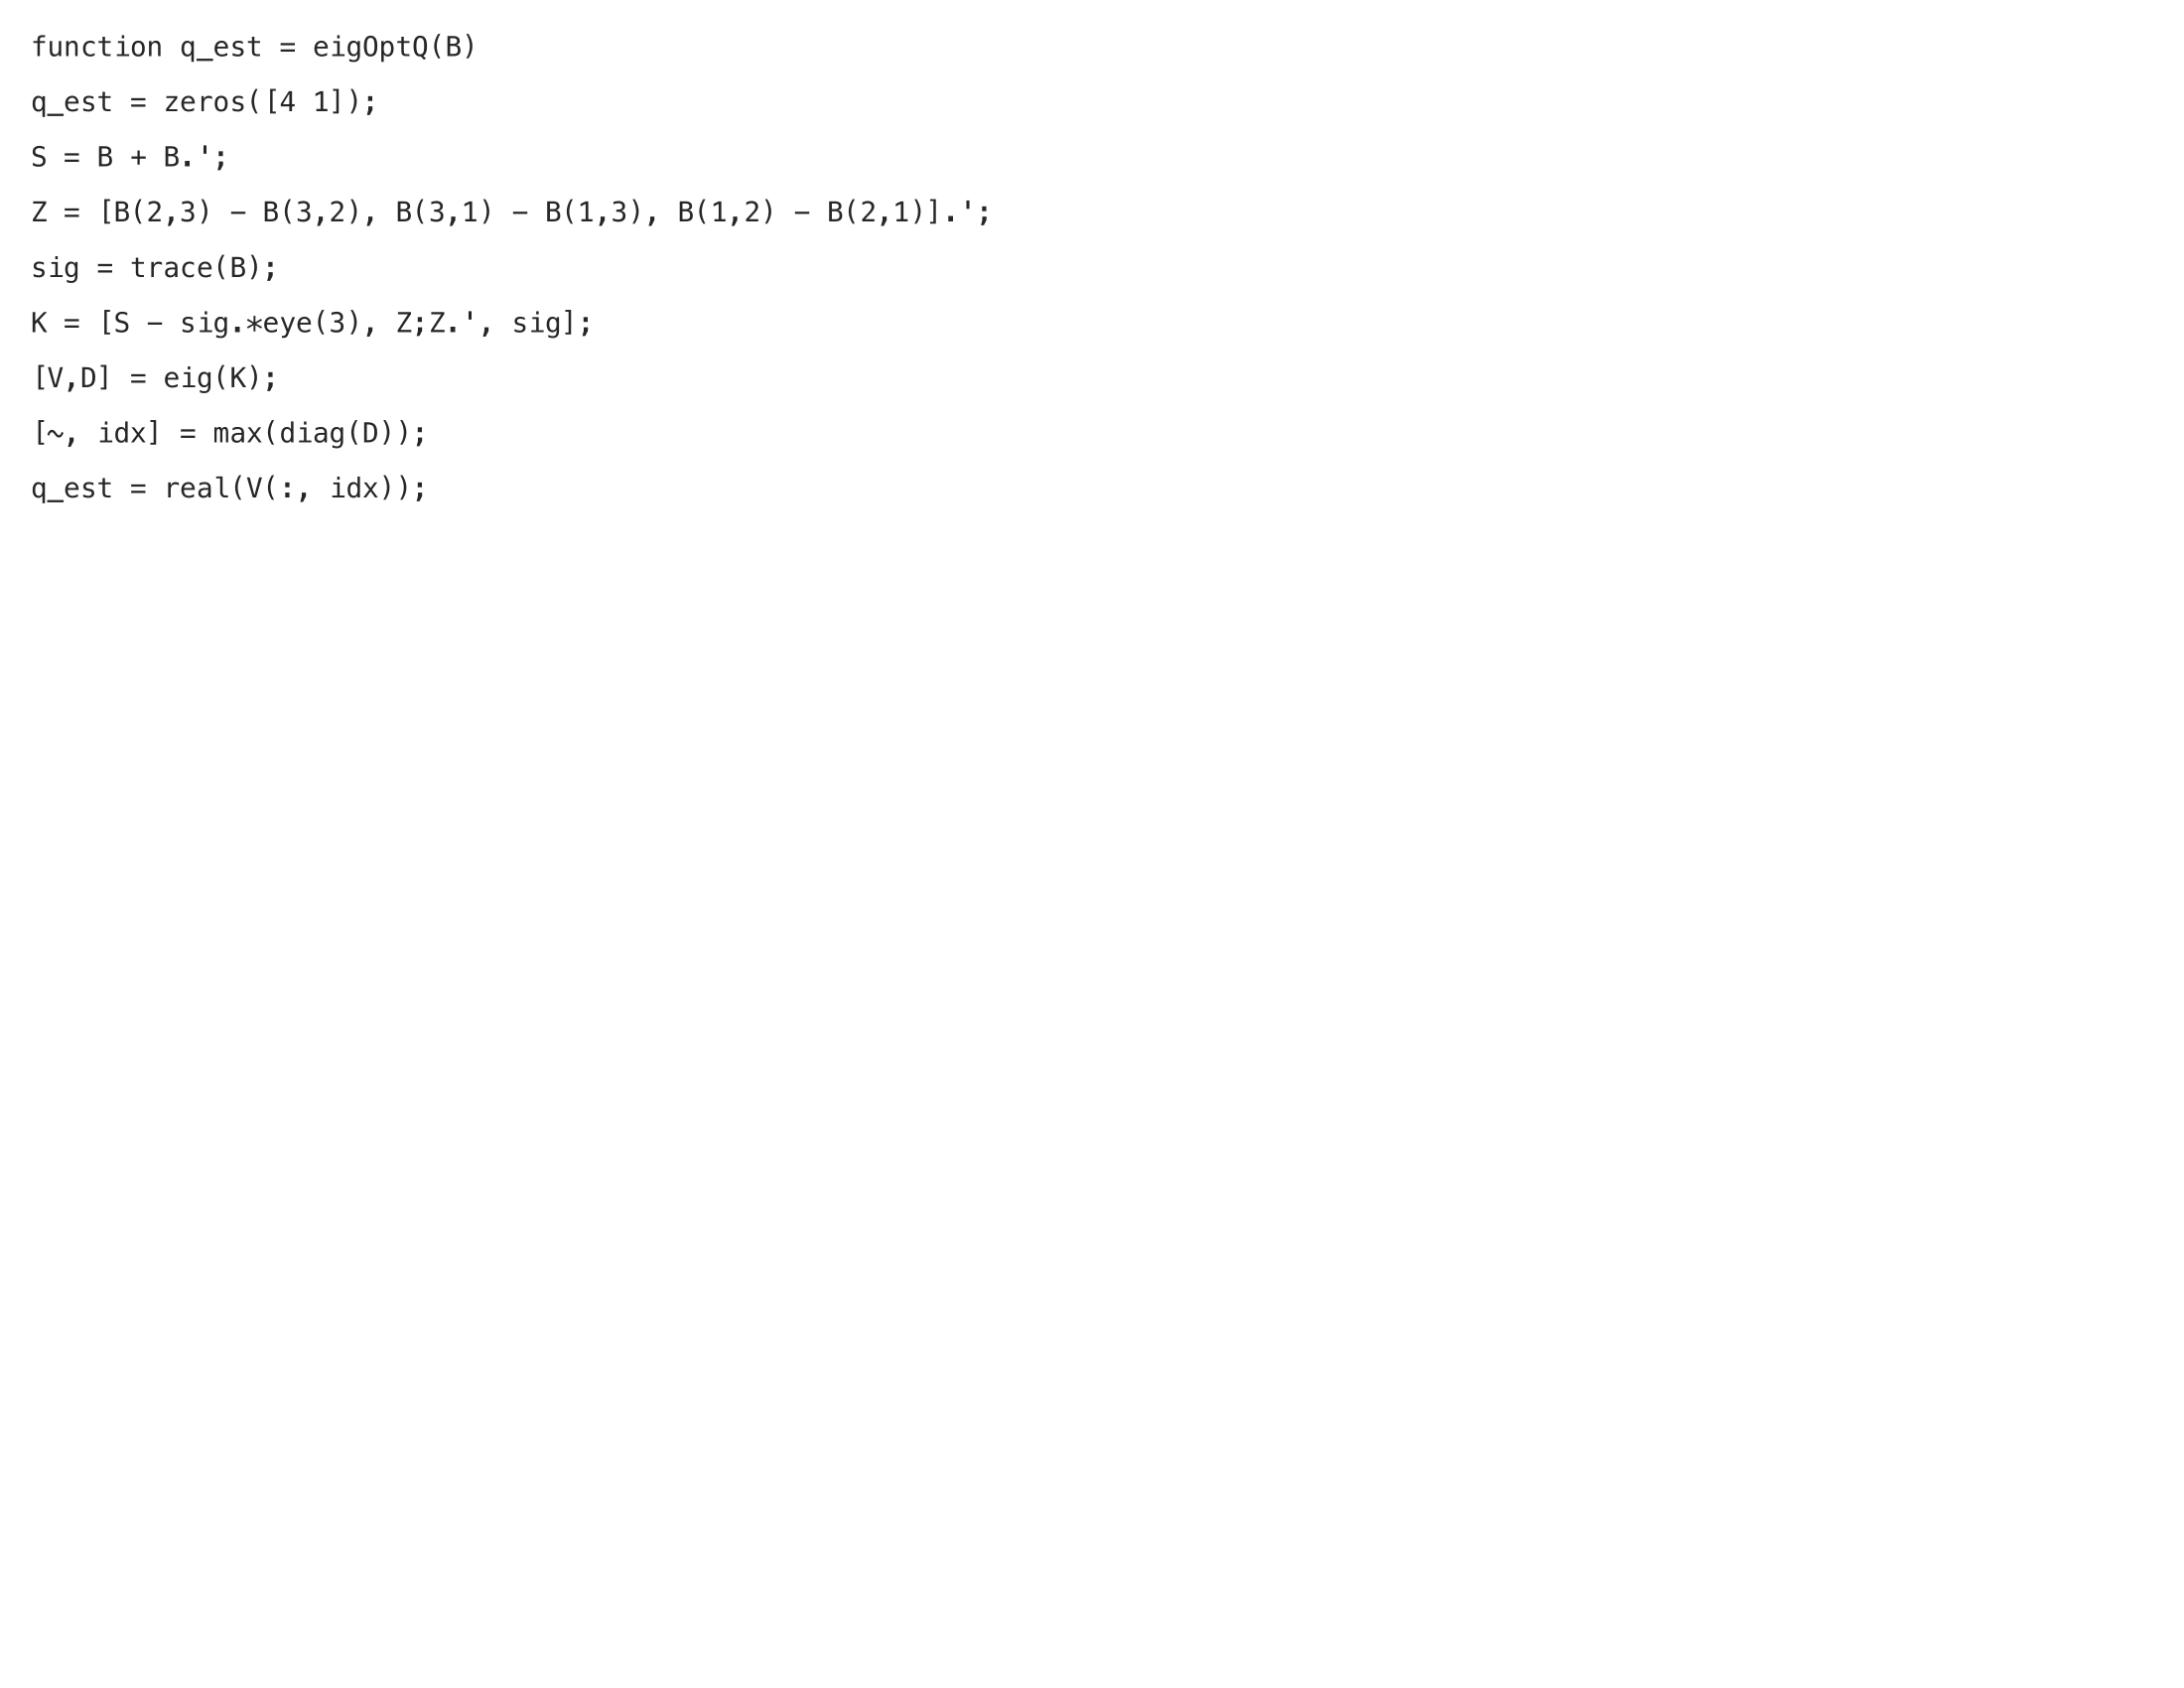
\includegraphics[trim={0cm 15cm 10cm 0cm},clip,width = 15cm]{Images/PS6/statisticalAttitude-2.png}
\end{figure}

\begin{figure}[H]
    \centering
    \captionsetup{ justification = centering }
    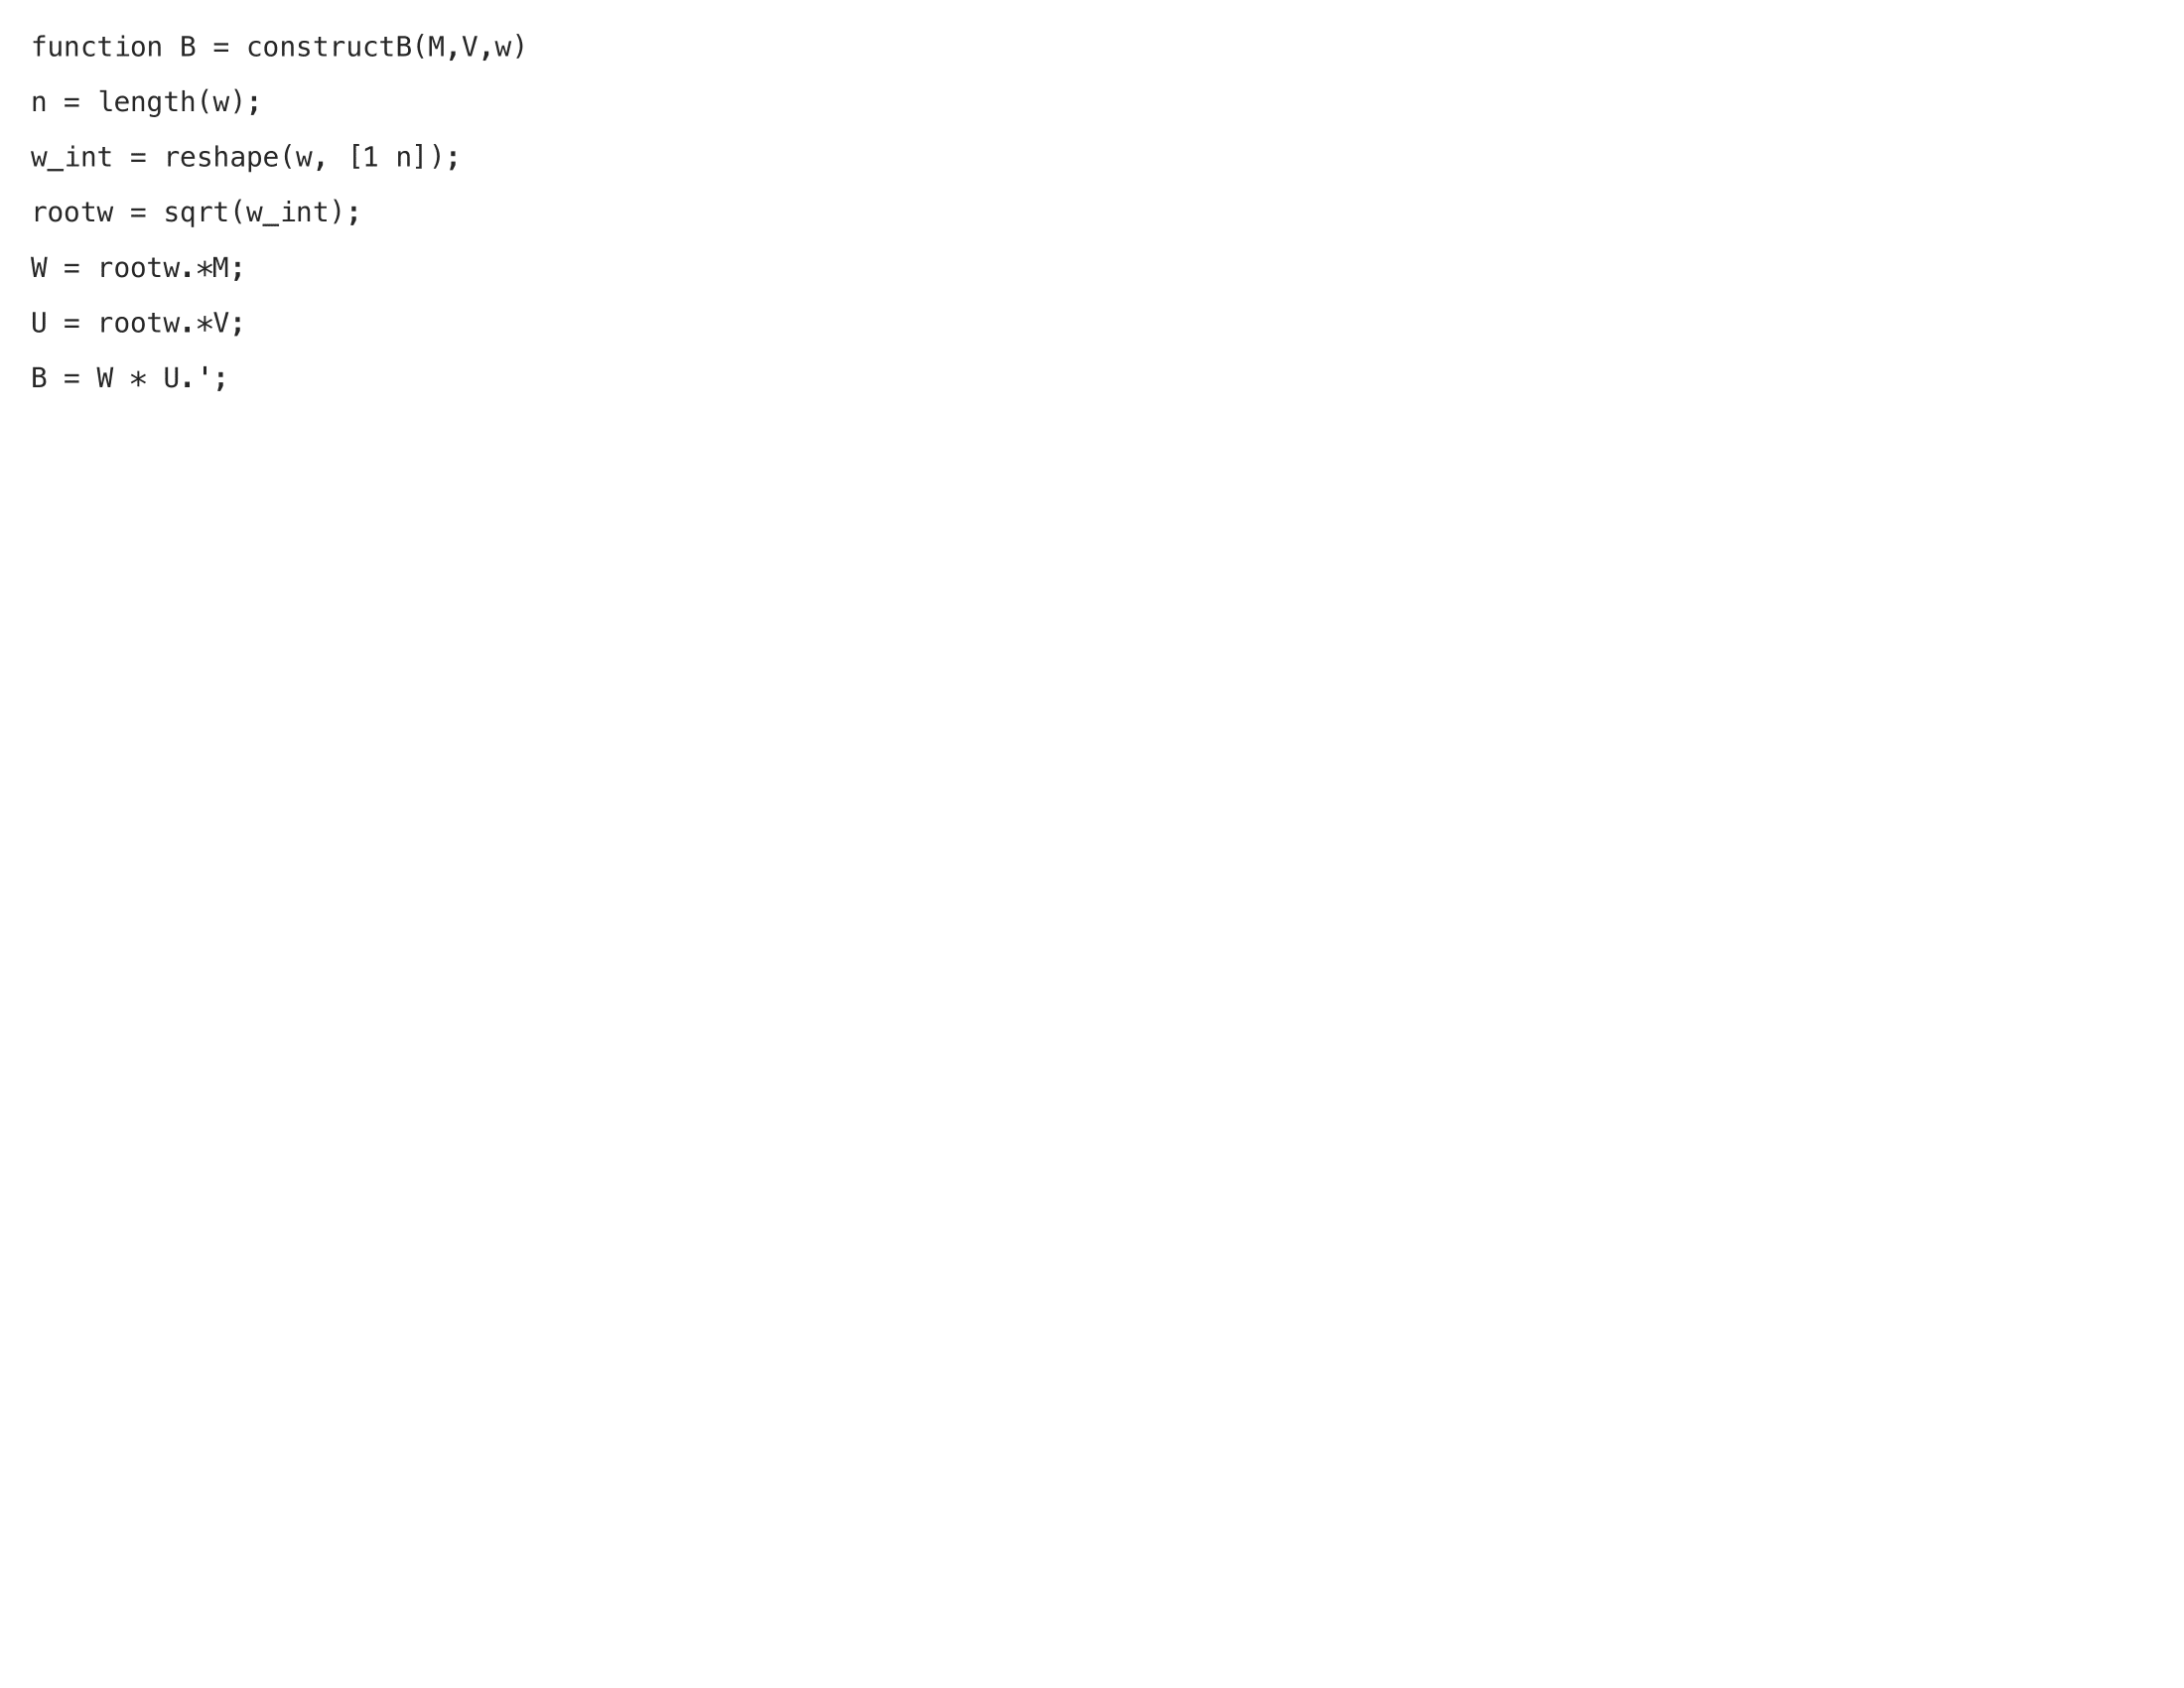
\includegraphics[trim={0cm 15cm 10cm 0cm},clip,width = 15cm]{Images/PS6/statisticalAttitude-3.png}
    \caption{Statistical Attitude Determination Model}
    \label{fig:stat_attitude}
\end{figure}

\subsubsection{Implement angular velocity measurements and the reconstruction of the attitude from those (through kinematic equations coded identically to ground truth but replicated in the spacecraft on- board computer)}

The reconstruction of the attitude from angular velocity measurements was obtained through copying the existing block to integrate the Euler equations into the on board computer (OBC). However, the angular velocity measurements were fed into the plant as opposed to a external torque. The resultant simulink diagrams are shown below.

\begin{figure}[H]
    \centering
    \captionsetup{ justification = centering }
    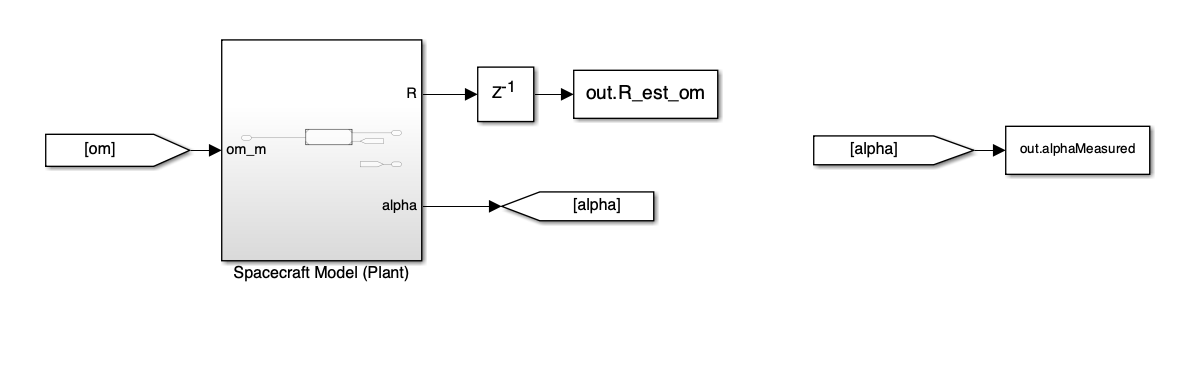
\includegraphics[width = 15cm]{Images/PS6/obc_plant_om.png}
    \caption{OBC Plant for $\omega$ Measurements}
    \label{fig:obc_plant_omega}
\end{figure}

\begin{figure}[H]
    \centering
    \captionsetup{ justification = centering }
    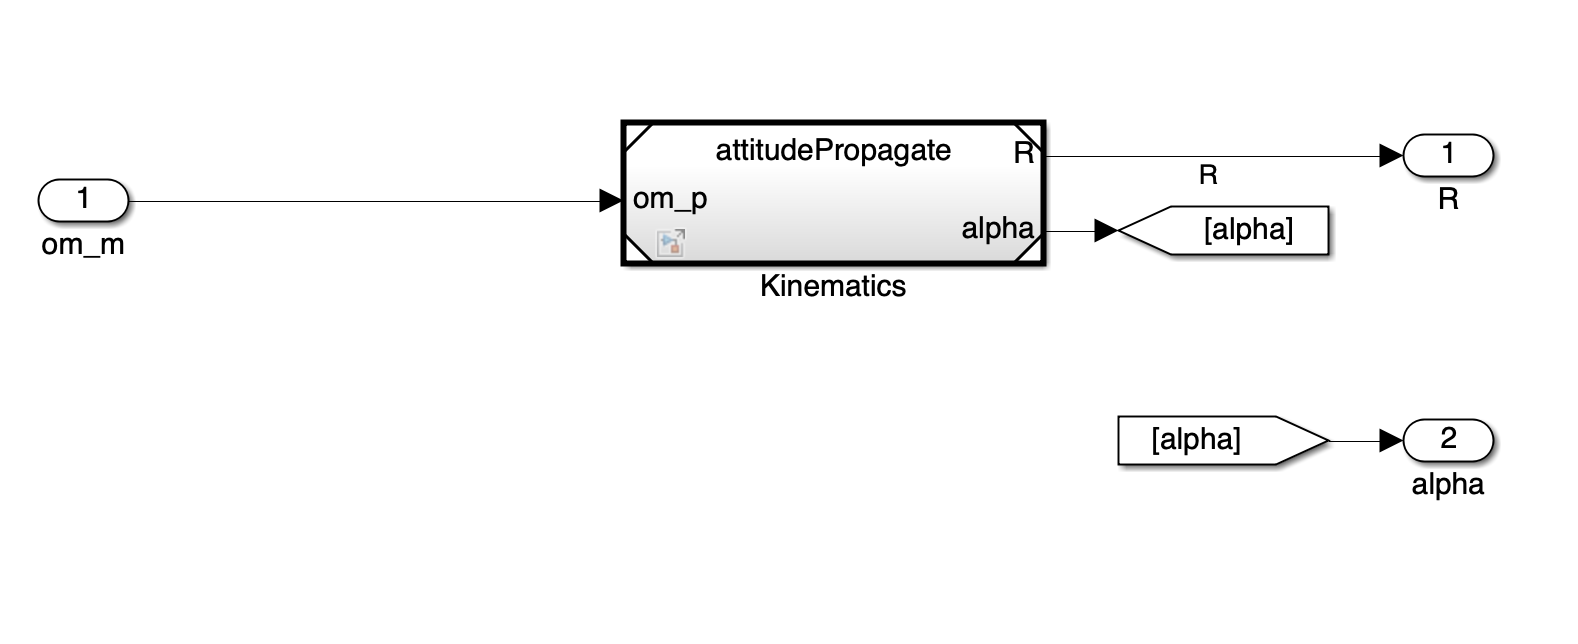
\includegraphics[width = 15cm]{Images/PS6/obc_attitudeProp_om.png}
    \caption{Attitude Propagator for $\omega$ Measurements in OBC}
    \label{fig:obc_prop_omega}
\end{figure}

The attitudePropagate block remained unchanged from previous work.

\subsection{Problem 6 - Plot the resulting estimated attitude in the absence of sensor errors. Show that it is identical to the true attitude (except for numerical errors).}

First, the deterministic attitude method was tested using the "undersampled" (2 available measurement) case. This was down with the feed through model. That is, no fictitious measurements were generated before creating a triad. The results of this simulation are seen in Figure \ref{fig:det_attitude_undersampled_default}.

\begin{figure}[H]
    \centering
    \captionsetup{ justification = centering }
    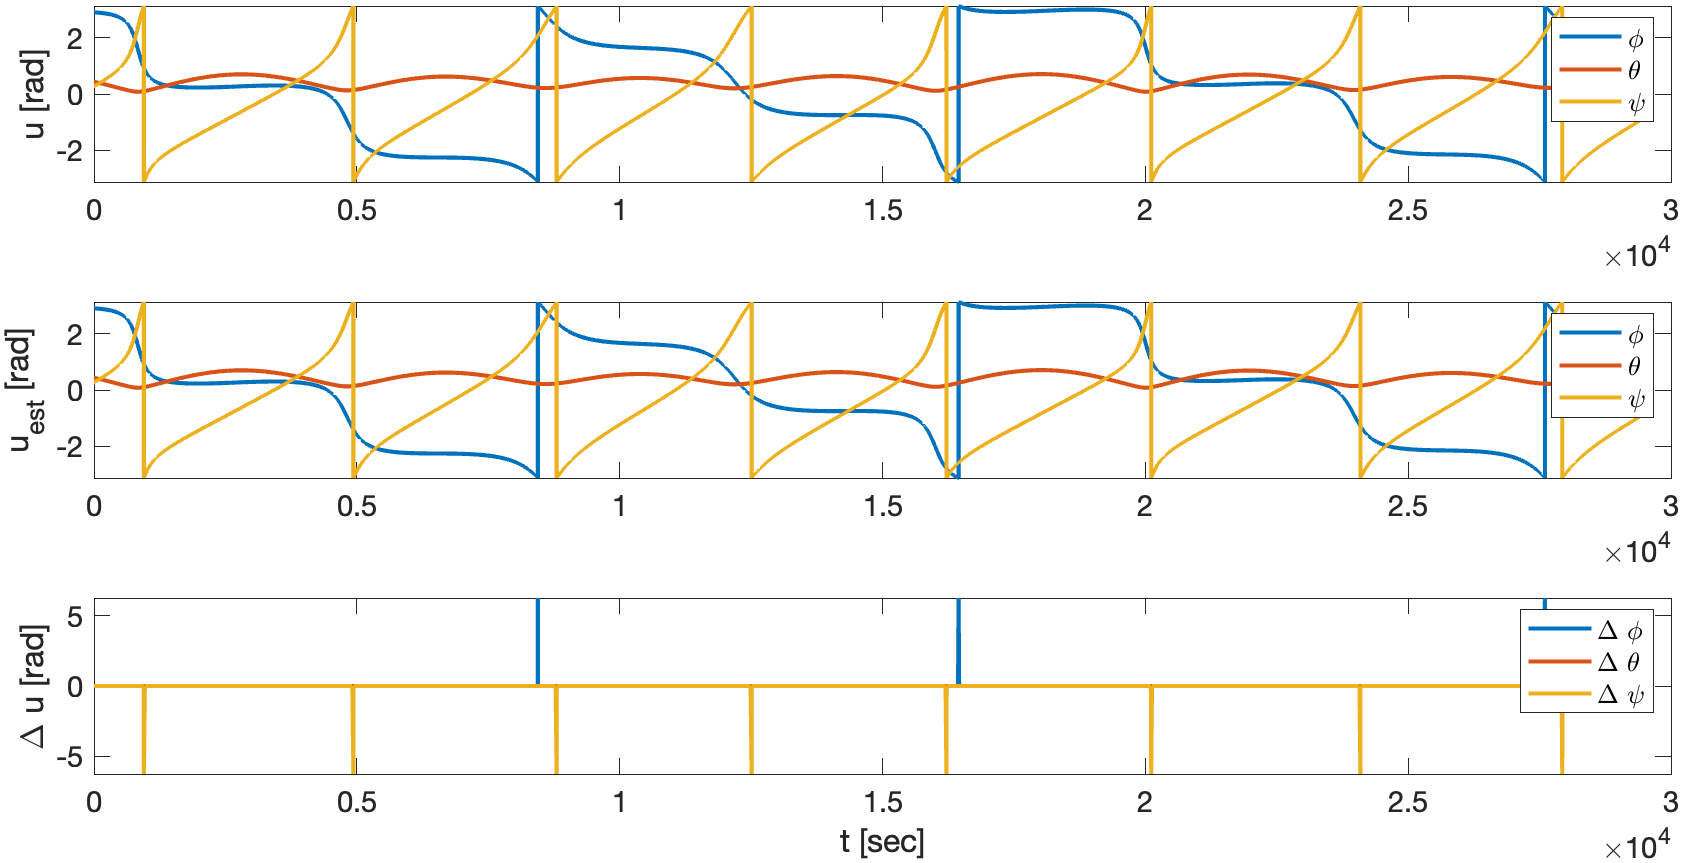
\includegraphics[width = 12cm]{Images/PS6/attitude_estimation_undersampled_det_default.png}
    \caption{Ground Truth vs. Estimated Attitude for Undersampled Deterministic Method with Feed Through Measurements}
    \label{fig:det_attitude_undersampled_default}
\end{figure}

The following test was deterministically performing attitude determination using fictitious measurements on the undersampled case. These results are seen below in Figure \ref{fig:det_attitude_undersampled_fictitious}. 

\begin{figure}[H]
    \centering
    \captionsetup{ justification = centering }
    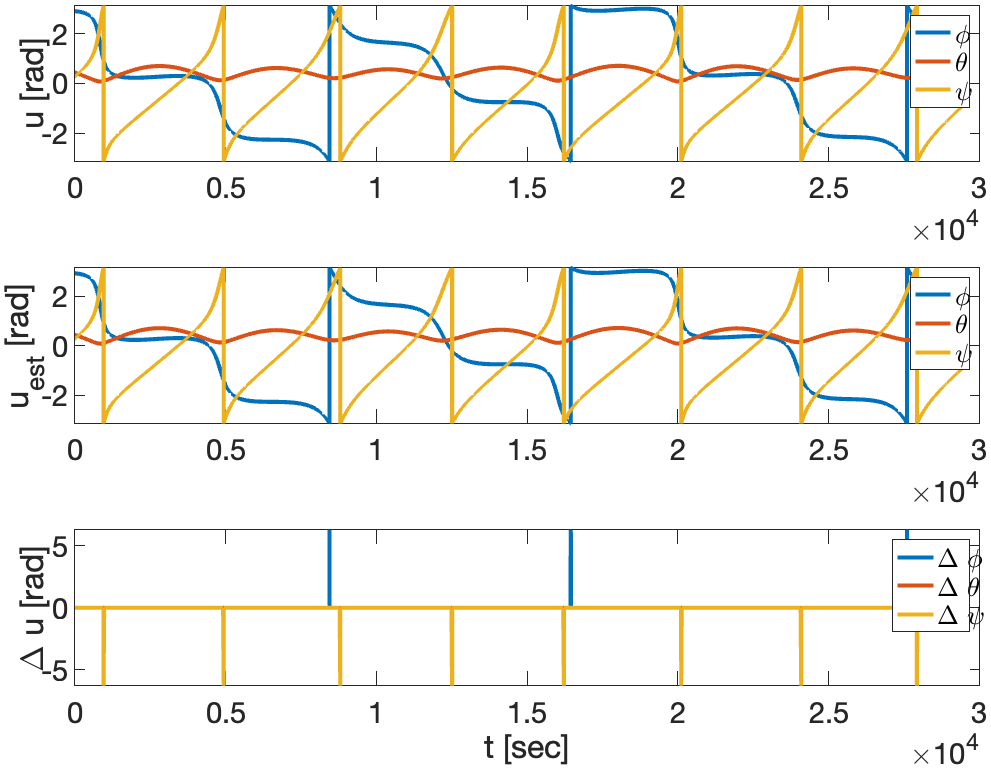
\includegraphics[width = 12cm]{Images/PS6/attitude_estimation_undersampled_det_fictitious.png}
    \caption{Ground Truth vs. Estimated Attitude for Undersampled Deterministic Method with Fictitious Measurements}
    \label{fig:det_attitude_undersampled_fictitious}
\end{figure}

The last undersampled case was on the statistical method with feed through on the measurements. These results are seen in Figure \ref{fig:stat_attitude_undersampled_default}.

\begin{figure}[H]
    \centering
    \captionsetup{ justification = centering }
    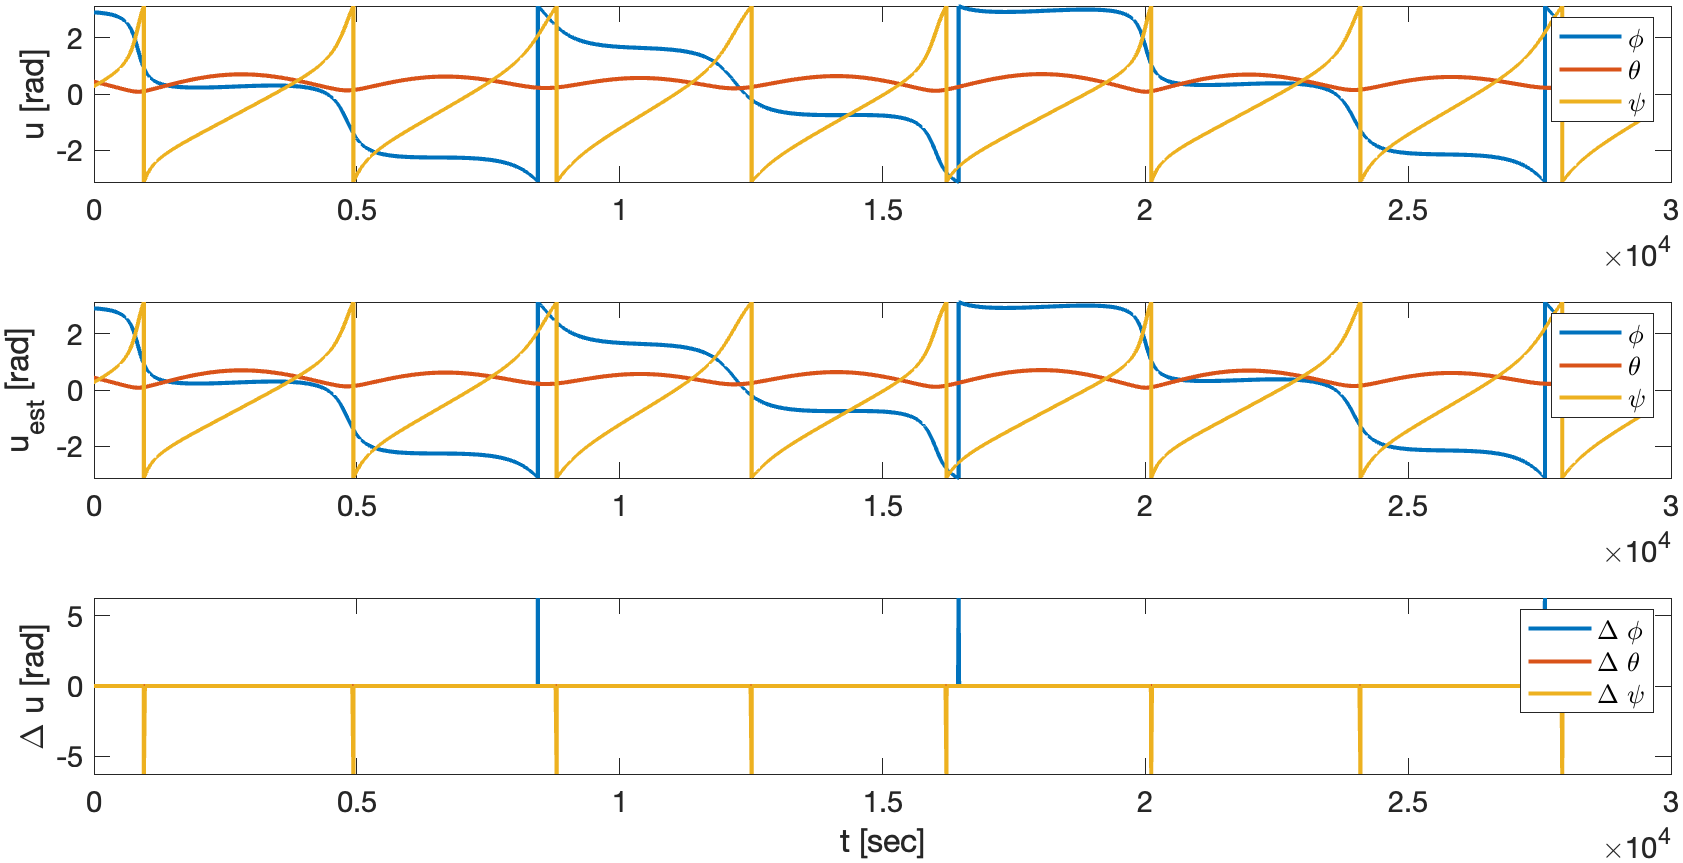
\includegraphics[width = 12cm]{Images/PS6/attitude_estimation_undersampled_q_default.png}
    \caption{Ground Truth vs. Estimated Attitude for Undersampled Statistical Method with Feed Through Measurements}
    \label{fig:stat_attitude_undersampled_default}
\end{figure}

The next step was to validate that both deterministic and statistical attitude determination methods were robust to oversampled measurements (i.e. 10 available measurements). The results of these for each respective method are shown in Figure \ref{fig:det_attitude_oversampled_default} and Figure \ref{fig:stat_attitude_oversampled_default}. 

\begin{figure}[H]
    \centering
    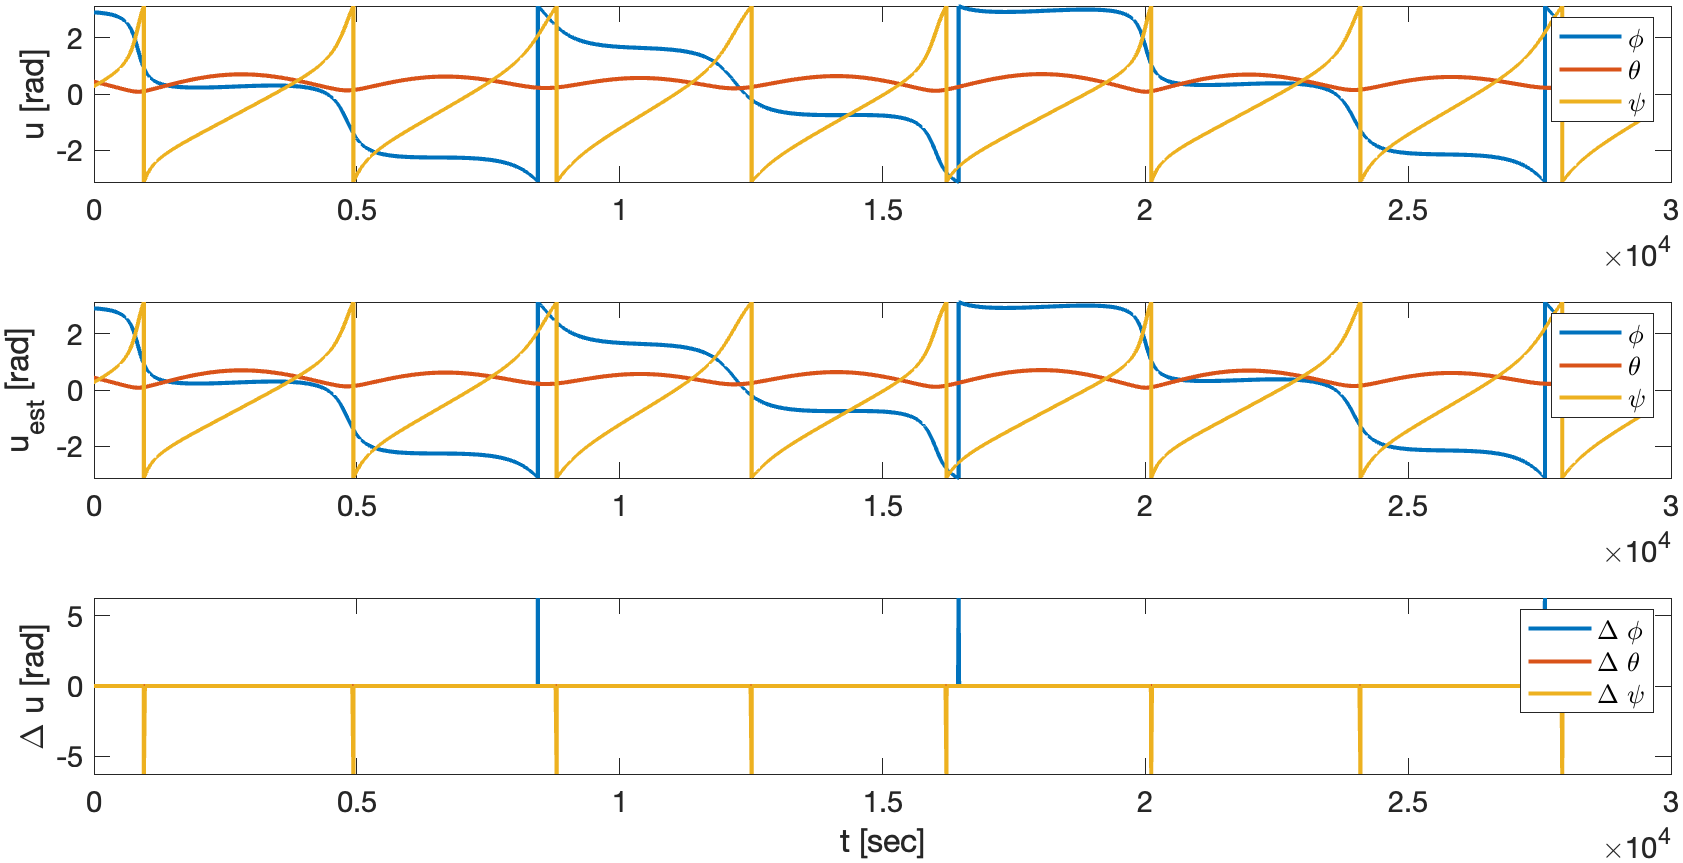
\includegraphics[width = 12cm]{Images/PS6/attitude_estimation_oversampled_det_default.png}
    \caption{Ground Truth vs. Estimated Attitude for Oversampled Deterministic Method with Feed Through Measurements}
    \label{fig:det_attitude_oversampled_default}
\end{figure}

\begin{figure}[H]
    \centering
    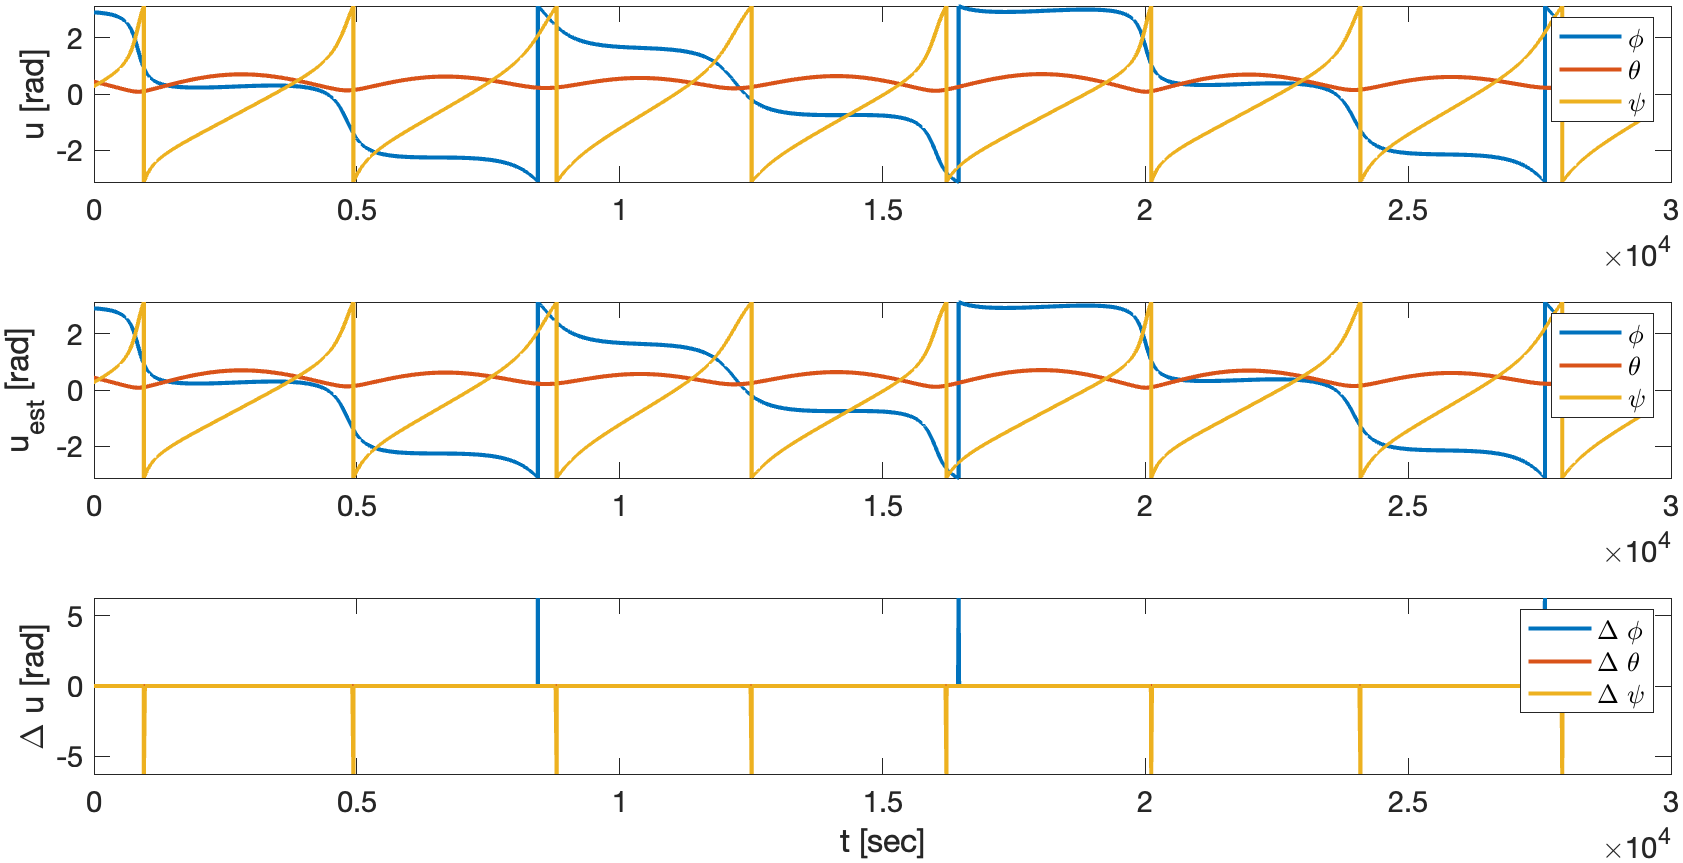
\includegraphics[width = 12cm]{Images/PS6/attitude_estimation_oversampled_q_default.png}
    \caption{Ground Truth vs. Estimated Attitude for Oversampled Statistical Method with Feed Through Measurements}
    \label{fig:stat_attitude_oversampled_default}
\end{figure}

For all cases it is seen that the error between the true state and the estimated state is nearly zero (i.e. on the order of $10^-4$). There are spikes in the error plot where singularities occur. A future fix for this might be to use quaternions or a different Euler angle sequence. 

To validate that the resultant Euler angles from the OBC $omega$ measurements were the same as the ground truth. They were co-plotted and are shown below in Figure \ref{fig:obcVsGroundOmega}.

\begin{figure}[H]
    \centering
    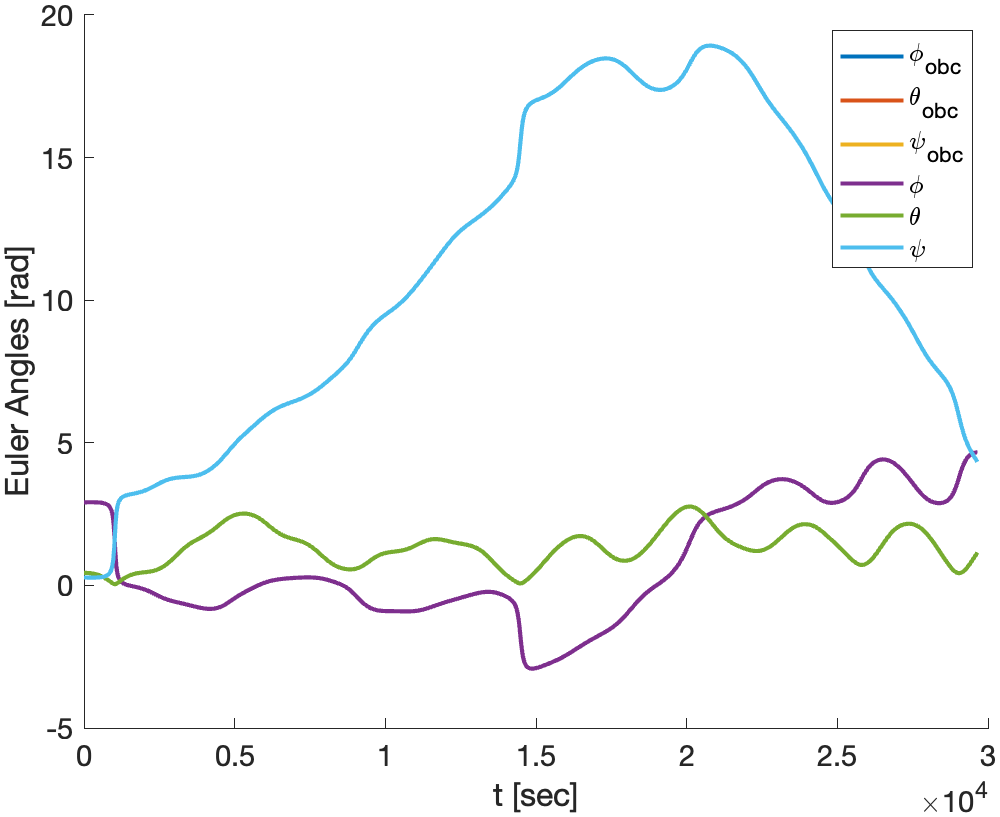
\includegraphics[width = 12cm]{Images/PS6/obcVsGroundOmegas.png}
    \caption{Ground Truth vs. Estimated Attitude for $\omega$ Measurements}
    \label{fig:obcVsGroundOmega}
\end{figure}

The plots for the ground trut perfectly overlayed those from the OBC.